\documentclass{report}
\usepackage{palatino, url, multicol}
\usepackage[utf8]{inputenc}
\usepackage[croatian]{babel}
\usepackage[T1]{fontenc}
\usepackage{graphicx}
\usepackage{booktabs}
\usepackage{amsmath}
\usepackage{amssymb}

\begin{document}

\tableofcontents
\newpage

\chapter{Maxwellove jednadžbe}

\section{Gaussov zakon za električno polje}
\small \textsc{Izvor:} \textit{predavanje (29.10.2007.), knjiga (Kulišić)}

Neka površina $S$ se nalazi u nekom električnom polju $\vec{E}$. Ako je $\vec{n}$ vektor normale površine, imamo $\vartheta = \angle \left( {\vec s,\vec D} \right)$, te vrijedi:
\begin{equation}
	\phi  = \varepsilon \vec{E} \vec{S} = \varepsilon _0 \varepsilon _r \vec{E} \vec{S} = \vec{D} \vec{S} = DS\cos \vartheta 
	\label{tok-opcenito}
\end{equation}
$\phi $ - Tok homogenog električnog polja kroz ravnu ploču.\\*
$\vec{D} $ - Vektor električnog pomaka.
$$\begin{array}{*{20}c}
  {D_x  = \frac{{Q_x }}
	{S}} & {D_y  = \frac{{Q_y }}
	{S}} & {D_z  = \frac{{Q_z }}
	{S}} & {D = \frac{1}
	{S}\sqrt {Q_x ^2  + Q_y ^2  + Q_z ^2 } }  \\
\end{array} $$

\section{Prva Maxwellova jednadžba - integralni oblik}
\small \textsc{Izvor:} \textit{predavanje (29.10.2007.), knjiga (Kulišić)}

Ako se u kugli radijusa $R$ nalazi pozitivni točkasti naboj $Q$, tada je tok kroz površinu $S$
$$\phi = 4\pi R^2 D$$
$$E = \frac{Q}{4\pi \varepsilon R^2} $$
$$D = \varepsilon E = \frac{Q}{4\pi R^2} $$
\begin{equation}
	\phi = 4\pi R^2 \cdot \frac{Q}{4\pi R^2} = Q
	\label{tok-polja-kroz-kuglinu-plohu}
\end{equation}

Uzmimo zatvorenu plohu proizvoljnog oblika, površine $S$. Budući da, općenito, električno polje nije konstantno u svim točkama plohe $S$, vrijedi:
$$\phi = \vec{D} _1 \cdot \Delta \vec{S} _1 + \vec{D} _2 \cdot \Delta \vec{S} _2 + \vec{D} _3 \cdot \Delta \vec{S} _3 + \cdots = \sum\limits_i {\vec D_i  \cdot \Delta \vec S_i } $$
Ako $\Delta S _i \to 0$
\begin{equation}
	\phi = \mathop {\lim }\limits_{\Delta \vec{S} _i \to 0 } \sum\limits_i {\vec D_i  \cdot \Delta \vec S_i } = \mathop{{\int\!\!\!\!\!\int}\mkern-21mu \bigcirc}\limits_s {\vec D \cdot d\vec S}
	\label{tok-polja-kroz-zatvorenu-plohu}
\end{equation}
Ako uvrstimo (\ref{tok-polja-kroz-kuglinu-plohu}) u (\ref{tok-polja-kroz-zatvorenu-plohu}), dobit ćemo \textsc{Gaussov zakon za elektrostatsko polje - osnovni zakon elektrostatike}
\begin{equation}
	\mathop{{\int\!\!\!\!\!\int}\mkern-21mu \bigcirc}\limits_s {\vec D \cdot d\vec S}  = Q
	\label{gaussov-zakon-za-elektrostatsko-polje}
\end{equation}
Ako naboj $Q$ izrazimo prostornom gustoćom naboja u volumenu $V$, imamo:
\begin{equation}
	Q = \iiint\limits_V {\varrho dV}
	\label{naboj-izrazen-prostornom-gustocom-naboja}
\end{equation}
Uvrstimo (\ref{naboj-izrazen-prostornom-gustocom-naboja}) u (\ref{gaussov-zakon-za-elektrostatsko-polje}):
\begin{equation}
	\mathop{{\int\!\!\!\!\!\int}\mkern-21mu \bigcirc}\limits_s {\vec D \cdot d\vec S}  = \iiint\limits_V {\varrho dV}
	\label{prva-maxwellova-jed-u-integralnom-obliku}
\end{equation}
To je \textit{prva} Maxwellova jednadžba u integralnom obliku.

\section{Prva Maxwellova jednadžba - diferencijalni oblik}
\small \textsc{Izvor:} \textit{predavanje (29.10.2007.), knjiga (Kulišić)}

Ako (\ref{prva-maxwellova-jed-u-integralnom-obliku}) podijelimo sa $\Delta V$, pri čemu $\Delta V \to 0$, dobijemo
$$\mathop {\lim }\limits_{\Delta V \to 0} \frac{1}
{{\Delta V}} \cdot \mathop{{\int\!\!\!\!\!\int}\mkern-21mu \bigcirc}\limits_s 
 {\vec Dd\vec S}  = \mathop {\lim }\limits_{\Delta V \to 0} \frac{1}
{{\Delta V}} \cdot \iiint\limits_V {\varrho dV}$$
Izračunajmo desnu stranu:
$$\mathop {\lim }\limits_{\Delta V \to 0} \frac{1}
{{\Delta V}} \cdot \iiint\limits_V {\varrho dV} = \varrho $$
Izraz
$$\mathop {\lim }\limits_{\Delta V \to 0} \frac{1}
{{\Delta V}} \cdot \mathop{{\int\!\!\!\!\!\int}\mkern-21mu \bigcirc}\limits_s 
 {\vec Dd\vec S} $$
je \textit{divergencija} od $\vec{D}$, te možemo pisati:
\begin{equation}
	div \vec{D} = \varrho 
	\label{prva-maxwellova-jed-u-diferencijalnom-obliku}
\end{equation}
To je \textit{prva} Maxwellova jednadžba u diferencijalnom obliku.

\subsection{Izračunavanje divergencije}
\small \textsc{Izvor:} \textit{predavanje (29.10.2007.), knjiga (Kulišić)}

\begin{equation}
	\mathop{{\int\!\!\!\!\!\int}\mkern-21mu \bigcirc}\limits_s {\vec Dd\vec S}
	\label{tok-vektora-d}
\end{equation}
možemo zapisati kao:
$$\begin{array}{*{20}l}
   {(\ref{tok-vektora-d})} & = & (D _x + dD _x)dydz - D _x dydz + (D _y + dD _y)dxdz - D _y dxdz + (D _z + dD _z)dxdy - D _z dxdy \\
   {} & = & dD _x dydz + dD _y dxdz + dD _z dxdy  \\
   {} & = & \frac{\partial D _x}{\partial x} dxdydz + \frac{\partial D _y}{\partial y} dxdydz + \frac{\partial D _z}{\partial z} dxdydz \\
   {} & = & \left ( \frac{\partial D _x}{\partial x} + \frac{\partial D _y}{\partial y} + \frac{\partial D _z}{\partial z} \right ) dV \\
\end{array}$$
Povežimo to sa \textit{prvom} Maxwellovom jednadžbom:
$$\mathop{{\int\!\!\!\!\!\int}\mkern-21mu \bigcirc}\limits_s {\vec D \cdot d\vec S}  = \iiint\limits_V {\varrho dV}$$
$$\frac{\partial D _x}{\partial x} + \frac{\partial D _y}{\partial y} + \frac{\partial D _z}{\partial z} = \varrho $$
Tako je u Cartesijevu koordinatnom sustavu:
$$div \vec{D} = \frac{\partial D _x}{\partial x} + \frac{\partial D _y}{\partial y} + \frac{\partial D _z}{\partial z} = \varrho $$
\begin{equation}
	\nabla \vec{D} = \varrho
	\label{gradijent-vektoraD}
\end{equation}

\section{Električni potencijal}
\small \textsc{Izvor:} \textit{predavanje (29.10.2007.), knjiga (Horvat)}

Imamo linijski integral od $A$ do $B$ električnog polja točkastog naboja $Q$
$$\int\limits_A^B {\vec{E} d \vec{l}} $$
Taj integral ne ovisi o putanji, već samo o krajnjim točkama, pa vrijedi:
$$\oint\limits_A^B {\vec{E}d \vec{l}} = 0$$
Dalje, imamo:
$$\vec{E}d \vec{l} = -dV(r)$$
$$\int\limits_A^B {\vec{E}d \vec{l}} = - \int\limits_A^B {dV(r)} = - \left[ {V(r_B ) - V(r_A )} \right]$$
$$V(r_B ) - V(r_A ) = - \int\limits_A^B {\vec{E}d \vec{l}}$$
$$V(r_B) = - \int\limits_A^B {\vec{E}d \vec{l}} + V(r_A )$$
$V(x,y,z)$ - Električni potencijal točke $(x,y,z)$ $[V]$

Uzmimo:
$$\left. {\begin{array}{*{20}c}
   {A \to \infty }  \\
   {V(r \to \infty ) = 0}  \\

 \end{array} } \right\}V(B) =  - \int\limits_\infty ^B {\vec Ed\vec l} $$
Za točkasti naboj vrijedi:
\begin{equation}
	V(r) = \frac{1}{4 \pi \varepsilon } \cdot \frac{Q}{r}
	\label{potencijal-tockastog-naboja}
\end{equation}

\section{Rad u električnom polju i potencijalna energija}
\small \textsc{Izvor:} \textit{predavanje (29.10.2007.), knjiga (Horvat)}

Ako imamo naboj $Q$ koji unutar električnog polja $\vec{E}$ putuje jednolikom brzinom od $A \to B$, vrijedi:
$$W _v = - \int \limits_A^B {Q \vec{E}d \vec{l}} = Q \left (V _B - V _A \right ) = Q \Delta V$$
\begin{equation}
	\Delta V = \frac{W _v}{Q}
	\label{razlika-potencijala-i-energija}
\end{equation}
$\Delta V$ - Razlika potencijala\\*
$W _v$ - Rad koji izvrši \textit{vanjska} sila

Iz teorema o kinetičkoj energiji i radu imamo: $W = \Delta E _k$. Budući da je $v = konst.$, slijedi $\Delta E _k = 0$, pa je \textit{vanjski} rad po iznosu jednak radu koji izvrši električno polje, ali je suprotnog predznaka.
$$W _E = \int \limits_A^B {Q \vec{E} d \vec{l}}$$
$W _E$ - Rad električnog polja

Ako dovedemo $Q$ iz $\infty $ u točku $A$, vrijedi:
$$W = Q \left (V(A) - V(\infty ) \right ) = - Q \int \limits_\infty ^A {\vec{E}d \vec{l}}$$
$$W = - \int \limits_\infty ^A {\vec{F}d \vec{l}}$$
$W$ - Elektrostatski potencijal

\section{Električna struja}
\small \textsc{Izvor:} \textit{predavanje (31.10.2007.)}\\*
\small \textsc{NAPOMENA:} \textbf{Izvod nisam našao u Kulišiću. Valjda je iz Horvata.}

$$\Delta V = S \Delta x \to n = n _0 \Delta V $$
$n _0$ - Broj slobodnih elektrona nosioca naboja $q$ u $1 m^3$
$$\Delta Q = nq = n _0 \Delta V q = S \Delta x n _0 q = S v _d \Delta t n _0 q $$
$$I = \frac{\Delta Q}{\Delta t} = n _0 q v _d S $$

\subsection{Gustoća struje}
\small \textsc{Izvor:} \textit{predavanje (31.10.2007.)}\\*
\small \textsc{Napomena:} \textbf{Izvod nisam našao u Kulišiću. Valjda je iz Horvata}

$$J = \frac{I}{S} = n _0 q v _d$$
$$\vec{J} = n _0 q \vec{v} _d$$

\subsection{Ohmov zakon}
\small \textsc{Izvor:} \textit{predavanje (31.10.2007.)}\\*
\small \textsc{Napomena:} \textbf{Izvod nisam našao u Kulišiću. Valjda je iz Horvata}

$$\vec{J} = \sigma \vec{E}$$
$\sigma $ - Električna vodljivost $[Siemens - S]$

Ako imamo vodič duljine $l$, razlika potencijala je:
$$\Delta V = E l \Rightarrow E = \frac{\Delta V}{l}$$
$$J = \sigma E = \sigma \frac{\Delta V}{l} \Rightarrow \frac{I}{S} = \sigma \frac{\Delta V}{l}$$
Specifični otpor:
$$\rho = \frac{1}{\sigma}$$
$$R = \rho \frac{l}{S}$$
Električni otpor je definiran sa:
$$R = \frac{1}{\sigma} \cdot \frac{l}{S} \Rightarrow R = \frac{\Delta V}{I}$$
$$I = \frac{\Delta V}{R}$$
$\Delta V$ - Razlika potencijala (napon)

\section{Druga Maxwellova jednadžba - integralni oblik}
\small \textsc{Izvor:} \textit{predavanje (31.10.2007.), knjiga (Kulišić)}

$$\phi _B = B \cdot S$$
$$B = \frac{\phi _B}{S}$$
$\phi _B$ - Skup silnica koje prolaze kroz plohu $S$

Ako silnice magnetskog polja nisu okomite na površinu $S$, uzmimo $\vartheta = \angle (\vec n, \vec B)$, te imamo:
$$\vec{S} = S \vec{n}$$
$\vec{n}$ - Vektor normale površine $S$
$$\phi _B = BS \cos \vartheta = \vec{B} \vec{S}$$
Općenito:
\begin{equation*} {
	\phi _B = \iint\limits_S {\vec Bd\vec S}
	\tag{$[Wb]$}
}
\end{equation*}

Po Gaussovom zakonu za magnetizam broj silnica koje ulaze u neku zatvorenu plohu jednak je broju silnica koje iz nje izlaze:
$$\mathop{{\int\!\!\!\!\!\int}\mkern-21mu \bigcirc}\limits_S {\vec Bd\vec S}  = 0$$
To je \textit{druga} Maxwellova jednadžba u integralnom obliku.

\section{Druga Maxwellova jednadžba - diferencijalni oblik}
\small \textsc{Izvor:} \textit{predavanje (31.10.2007.), knjiga (Kulišić)}

\textit{Izvod je analogan izvodu za prvu Maxwellovu jednadžbu.}
$$div \vec{B} = 0$$
$$\nabla \vec{B} = 0$$
$$\frac{\partial B _x}{\partial x} + \frac{\partial B _y}{\partial y} + \frac{\partial B _z}{\partial z} = 0$$
To je \textit{druga} Maxwellova jednadžba u diferencijalnom obliku.

\section{Lorentzova sila}
\small \textsc{Izvor:} \textit{predavanje (31.10.2007.)}\\*
\small \textsc{Napomena:} \textbf{Izvod nisam našao u Kulišiću. Valjda je iz Horvata}

Imamo naboj $Q$ koji se giba brzinom $v$ u magnetskom polju.\\*
Pokusi su pokazali:
\begin{center} {
	$F _m \sim Qv$\\*
	$F _m \sim B$\\*
	$\vec{F} _m \bot \vec{v}, \: \vec{F} _m \bot \vec{B}$\\*
	Smjer $\vec{F} _m$ na pozitivan naboj je\\* suprotan smjeru magnetske sile na negativan naboj.\\*
	$F _m \sim \sin \vartheta, \: \vartheta = \angle (\vec{v}, \vec{B})$
	}
\end{center}
$\vec{F} _m$ - Magnetska sila

Iz toga imamo:
$$\vec{F} _m = Q \vec{v} \times \vec{B}$$
$$F _m = QvB \sin \vartheta $$
Lorentzova sila:
$$\vec{F} _L = \vec{F} _e + \vec{F} _m = Q \vec{E} + Q \vec{v} \times \vec{B}$$
$\vec{F} _m$ ne vrši rad pri premještanju naboja.
$$W = \vec{F} _m d\vec{l} = \vec{F} _m \vec{v} dt = Q(\vec{v} \times \vec{B}) \vec{v}dt = 0$$

\section{Sila na vodič u magnetskom polju}
\small \textsc{Izvor:} \textit{predavanje (31.10.2007.)}\\*
\small \textsc{Napomena:} \textbf{Izvod nisam našao u Kulišiću. Valjda je iz Horvata}

$$\vec{F}_m = q \vec{v}_d \times \vec{B}$$
$\vec{v}_d$ - Brzina naboja $q$ u vodiču
$$dV = Sdl \to dQ = nqSdl$$
$$I = nqv_dS$$
$$d\vec{F} = (q \vec{v}_d \times \vec{B}) n S \, dl = Id \vec{l} \times \vec{B}$$
$$\vec{F} = I \int \limits_A^B {d\vec{l} \times \vec{B}}$$
$$\vec{F} = \int \limits_A^B {(\vec{I} \times \vec{B})dl}$$
$$\vec{F} = I \int \limits_A^B {(d\vec{l} \times \vec{B})} = I \overrightarrow {AB} \times \vec{B}$$
$\overline {AB} $ - Dužina vodiča kojeg promatramo

Ukupna sila na zatvoreni vodič kojim teče struje je jednaka $0$.

\section{Definicija ampera (pokus)}
\small \textsc{Izvor:} \textit{predavanje (31.10.2007.)}\\*
\small \textsc{Napomena:} \textbf{Nisam našao u Kulišiću. Valjda je iz Horvata}

Imamo dva ravna paralelna vodiča.\\*
Svaki vodič stvara magnetsko polje $B$ na drugi vodič.
$$\begin{array}{*{20}c}
   {F} \hfill & {=} \hfill & {I_1 B_2 l} \hfill  \\
   {} \hfill & {=} \hfill & {I_1 \cdot \mu_0 \cdot \frac{I _2}{2 \pi d} \cdot l} \hfill  \\
   {} \hfill & {=} \hfill & {I_1 \cdot \frac{2 \mu _0 I_2}{4 \pi d} \cdot l} \hfill  \\
	 {} \hfill & {=} \hfill & {2 \frac{\mu _0}{4 \pi} \cdot l \cdot \frac{I_1 I_2}{d}} \hfill  \\
 \end{array} $$
 
Ako podesimo:
$$\left. {\begin{array}{*{20}c}
   {I_1 = I_2 = I}  \\
   {\frac{F}{l} = 2 \cdot 10^{-7} \frac{N}{m}}  \\
   {d = 1 m}  \\

 \end{array} } \right\}{\text{vodičem teče struja od } 1\:A}$$
$$\frac{\mu _0}{4 \pi} = 10^{-7} \frac{Wb}{Am}$$
$[Wb]$ - Jedinica za magnetski tok

\section{Elektromagnetska indukcija}
\small \textsc{Izvor:} \textit{predavanje (31.10.2007.)}\\*
\small \textsc{Napomena:} \textbf{Nisam našao u Kulišiću. Valjda je iz Horvata}

$$\vec{F} _m = q \vec{v} \times \vec{B}, \: F _m = qvB$$
Ako je:\\*
$F_e = F_m$\\*
$qE = qvB$\\*
$E = vB$\\*
$\Delta V = El = Blv$\\*
Inducirana elektromotorna sila:
$$EMS _i = \varepsilon _i$$
$$W = Fl = qvBl$$
$$\varepsilon _i = \frac{W}{q} = Blv$$
$$\varepsilon _i = \vec{l}(\vec{v} \times \vec{B})$$

\section{Treća Maxwellova jednadžba - integralni oblik}
\small \textsc{Izvor:} \textit{predavanje (31.10.2007.), knjiga (Kulišić)}

\subsection{Faradayev zakon indukcije}
\small \textsc{Izvor:} \textit{predavanje (31.10.2007.), knjiga (Kulišić)}

U prisutnosti magnetskog polja, mehanička energija se pretvara u električnu.
$$\varepsilon = - \frac{d \phi}{dt}$$
$$\varepsilon = - N \frac{d \phi}{dt}$$
$N \phi$ - Ukupni tok (označava se sa $\psi $).\\*
Negativan predznak je posljedica zakona o očuvanju energije (\textsc{Lenzovo pravilo}).

Dok se vodič giba u magnetskom polju na njegove elektrone djeluje Lorentzova sila $F$ i tjera ih prema jednom kraju žice.
$$\vec{F} = -e \vec{v} \times \vec{B}$$
Inducirano elektrostatsko električno polje
$$\vec E _{ind} = \frac{\vec{F}}{Q}$$
$$\vec E _{ind} = \frac{\vec{F}}{-e} = \vec{v} \times \vec{B}$$
Vodič se polarizira, te razdvojeni naboji stvaraju u žici polje $\vec{E}$
$$\vec{E} = - \vec{v} \times \vec{B}$$
Inducirana elektromotorna sila jednaka je cirkulaciji induciranog polja:
$$\varepsilon _{ind} = \oint{\vec{E} _{ind}d \vec{s}} = \int \limits_C^D {(\vec{v} \times \vec{B} )d \vec{s}} = vBl \sin \left (\frac{\pi}{2} \right ) = vBl$$
Ako je $\vartheta = \angle (\vec{v}, \vec{B})$
$$\varepsilon _{ind} = vBl \sin \vartheta $$
Gibanjem vodiča za vrijeme $dt$ pređemo put $ds$:
$$ds = vdt$$
Pritom se površina promjeni za $lvdt$, pa je promjena magnetskog toka:
$$d \phi = B l v dt$$
Slijedi:
$$\frac{d \phi}{dt} = Blv$$
$$\varepsilon _{ind} = - \frac{d \phi}{dt}$$
\textsc{Faradayev zakon indukcije} općenito:
$$\varepsilon _{ind} = \oint\limits_K {\vec Ed\vec s} $$
$$\phi = \iint\limits_S {\vec Bd\vec S}$$
$$\oint\limits_K {\vec Ed\vec s} = - \frac{d}{dt} \left ( \iint\limits_S {\vec Bd\vec S}  \right )$$
Magnetski tok se može mijenjati na dva načina:
\begin{itemize}
 \item Mijenjanjem $\phi $ zbog vremenske promjene $\vec{B}$ u mirnoj petlji ($\frac{\partial \phi}{\partial t}$).
 \item Mijenjanjem $\phi $ zbog promjene površine petlje:
\end{itemize}
$$\oint\limits_K {\left( {\vec v \times \vec B} \right)d\vec s} $$
\begin{equation}
	\oint\limits_K {\vec E d\vec s} = - \frac{d \phi}{dt} = - \frac{\partial  \phi}{\partial t} - \oint\limits_K {\left( {\vec v \times \vec B} \right)d\vec s}
	\label{faradayev-zakon-opcenito}
\end{equation}
(\ref{faradayev-zakon-opcenito}) je općeniti izraz za Faradayev zakon indukcije.\\*
U elektrostatici vrijedi:
$$\oint\limits_K {\vec E d\vec s} = 0$$

\subsection{Lenzovo pravilo}
\small \textsc{Izvor:} \textit{predavanje (31.10.2007.), knjiga (Kulišić)}

$$\varepsilon = - \frac{d \phi}{dt}$$
$$I = \frac{\varepsilon}{R} = - \frac{1}{R} \cdot \frac{d \phi}{dt}$$

Predznak minus se objašnjava Lenzovim pravilom: \textit{inducirana} električna 
struja ima takav smjer da proizvodi tok koji se suprotstavlja promjeni toka zbog 
kojeg je nastala. Pravilo proizlazi iz zakona o očuvanju energije.

\subsection{Zaključni dio}
\small \textsc{Izvor:} \textit{predavanje (31.10.2007.), knjiga (Kulišić)}

Iz Faradayeva zakona indukcije imamo:
$$\varepsilon = - \frac{d \phi _B}{dt}$$
To možemo zapisati u obliku:
$$\oint\limits_K {\vec E d\vec s} = - \frac{d} {{dt}}\iint\limits_S {\vec Bd\vec S}$$
To je \textit{treća} Maxwellova jednadžba u integralnom obliku.

\section{Treća Maxwellova jednadžba - diferencijalni oblik}
\small \textsc{Izvor:} \textit{predavanje (5.11.2007.), knjiga (Kulišić)}

$$\oint\limits_K {Ed\vec s} = - \frac{d}{dt} \iint \limits_S \vec{B} d \vec{S}$$
Podijelimo sve sa $\Delta S$, $\Delta S \to 0$:
\begin{equation}
	\mathop {\lim }\limits_{\Delta S \to 0} \frac{1}
	{{\Delta S}}\oint\limits_K {Ed\vec s}  =  - \mathop {\lim }\limits_{\Delta S \to 0} \frac{d}
	{{dt}}\left( {\frac{1}
	{{\Delta S}}\iint\limits_S {Bd\vec S}} \right)
	\label{maxwell-diff-limes}
\end{equation}
Radi jednostavnosti promatrajmo površinu $\Delta S$ kao infinitezimalno mali kvadrat, a krivulja $K$ opseg kvadrata $ABCD$.
$$\oint\limits_{ABCD} {\vec E d \vec s} = \int\limits_{AB} {\vec E d \vec s} + \int\limits_{BC} {\vec E d \vec s} + \int\limits_{CD} {\vec E d \vec s} + \int\limits_{DA} {\vec E d \vec s}$$
$$\int\limits_{AB} {\vec E d \vec s} + \int\limits_{CD} {\vec E d \vec s} = \left [ E_y(z) - E_y(z + dz) \right ] dy = - \frac{\partial E_y}{\partial z} dz dy$$
$$\int\limits_{BC} {\vec E d \vec s} + \int\limits_{DA} {\vec E d \vec s} = \left [ E_z(y + dy) - E_z(y) \right ] dz = \frac{\partial E_z}{\partial y} dz dy$$
\begin{equation}
	\oint \limits_{ABCD} {\vec E d \vec s} = \left ( \frac{\partial E_z}{\partial y} - \frac{\partial E_y}{\partial z} \right )dz dy
	\label{cirkulacija-vektora-E}
\end{equation}
Magnetski tok kroz $dS$ je:
\begin{equation}
	\iint \limits_{dS} {\vec B d \vec S} = B_x dz dy
	\label{magnetski-tok-kroz-dS}
\end{equation}
Uvrstimo (\ref{cirkulacija-vektora-E}) i (\ref{magnetski-tok-kroz-dS}) u (\ref{maxwell-diff-limes}):
$$\frac{\partial E_z}{\partial y} - \frac{\partial E_y}{\partial z} = - \frac{\partial B_x}{\partial t}$$
Integracijom po ostalim stranicama dobivamo:
$$\frac{\partial E_y}{\partial x} - \frac{\partial E_x}{\partial y} = - \frac{\partial B_z}{\partial t}$$
$$\frac{\partial E_x}{\partial z} - \frac{\partial E_z}{\partial x} = - \frac{\partial B_y}{\partial t}$$
Te skalarne veličine možemo prikazati jednom vektorom, koji ćemo nazvati \textit{rotacija električnog polja}
$\vec{E}$ ($rot \vec{E}$), koji je definiran izrazom:
$$\vec{n} \cdot rot \vec E = \mathop {\lim }\limits_{\Delta s \to 0} \frac{1} {{\Delta s}}\oint\limits_K {\vec Ed\vec s} $$
$rot \vec E$ ove komponente:
$$(rot \vec E)_x = \frac{\partial E_z}{\partial y} - \frac{\partial E_y}{\partial z}$$
$$(rot \vec E)_y = \frac{\partial E_x}{\partial z} - \frac{\partial E_z}{\partial x}$$
$$(rot \vec E)_z = \frac{\partial E_y}{\partial x} - \frac{\partial E_x}{\partial y}$$
\textit{Treća} Maxwellova jednadžba u diferencijalnom obliku:
\begin{equation}
	rot \vec E = - \frac{\partial \vec B}{\partial t}
	\label{treca-maxwellova-jed-u-diff-obliku}
\end{equation}
$$\vec \nabla \times \vec E = - \frac{\partial \vec B}{\partial t}$$

\section{Četvrta Maxwellova jednadžba - integralni oblik}
\small \textsc{Izvor:} \textit{predavanje (5.11.2007.), knjiga (Kulišić)}

\subsection{Amp\'{e}reov zakon}
\small \textsc{Izvor:} \textit{predavanje (5.11.2007.), knjiga (Kulišić)}

Cirkulacija vektora jakosti magnetskog polja po krivulji $K$:
$$\oint\limits_K {\vec H d \vec s}$$
Ako promatramo magnetsko polje dugog ravnog vodiča kojim teče struja $I$, a krivulja je 
kružnica, tada je magnetsko polje $H = \frac{I}{2 \pi r}$, slijedi:
$$\oint\limits_K {\vec H d \vec s} = \oint\limits_K {\frac{I}{2 \pi r} d \vec s} = \frac{I}{2 \pi r} \oint\limits_K {d \vec s}$$
Putanja po kružnici je jednaka opsegu ($2 \pi r$), pa slijedi:
$$\oint\limits_K {\vec H d \vec s} = I$$
Ako krivulja obuhvaća više struja, možemo pisati:
$$\oint\limits_K {\vec H d \vec s} = \sum{I}$$
ili
$$\oint\limits_K {\vec B d \vec s} = \mu \sum{I}$$
To je Amp\'{e}rov zakon ili \textit{zakon protjecanja}.

\subsection{Struja pomaka}
\small \textsc{Izvor:} \textit{predavanje (5.11.2007.), knjiga (Kulišić)}

Provodna struja jednaka je struji pomaka:
\begin{equation}
	I_{pr} = \frac{dQ}{dt} = I_{pom}
	\label{jednakost-struja-provodna-i-pomaka}
\end{equation}
$I_{pr}$ - Provodna struja.\\*
$I_{pom}$ - Struja pomaka\\*
Prema Gaussovom zakonu je:
\begin{equation}
	\mathop{{\int\!\!\!\!\!\int}\mkern-21mu \bigcirc}\limits_S {\vec Dd\vec S} = Q
	\label{gaussov-zakon}
\end{equation}
Uvrstimo (\ref{gaussov-zakon}) u (\ref{jednakost-struja-provodna-i-pomaka}):
$$I_{pom} = \frac{d}{dt}\mathop{{\int\!\!\!\!\!\int}\mkern-21mu \bigcirc}\limits_S {\vec Dd\vec S} = \frac{d \phi _D}{dt}$$
To je ukupna struja pomaka kroz zatvorenu površinu oko ploće.\\*
Struja pomaka kroz odabranu površinu $S$ je:
$$I_{pom} = \frac{d}{dt} \iint\limits_S {\vec D d \vec S}$$
U Amp\'{e}reov zakon moramo uključiti obje struje:
$$\oint\limits_K {\vec H d \vec s} = I_{pr} + I_{pom}$$
\begin{equation}
	\oint\limits_K {\vec H d \vec s} = I + \frac{d}{dt} \iint\limits_S {\vec D d \vec S}
	\label{poopceni-amperov-zakon}
\end{equation}
$K$ - Rub plohe $S$ (krivulja).\\*
To je \textit{poopćeni Amp\'{e}reov zakon}.

\subsection{Zaključni dio}
\small \textsc{Izvor:} \textit{predavanje (5.11.2007.), knjiga (Kulišić)}

Izrazimo struju $I$ preko gustoće $\vec J$.
$$I = \iint\limits_S {\vec J d \vec S}$$
Uvrstimo to u (\ref{poopceni-amperov-zakon}), te dobijemo:
\begin{equation}
	\oint\limits_K {\vec H d \vec s} = \iint\limits_S {\vec J d \vec S} + \frac{d}{dt} \iint\limits_S {\vec D d \vec S}
	\label{cetvrta-maxwellova-jednadzba-int}
\end{equation}
To je \textit{četvrta} Maxwellova jednadžba u integralnom obliku.\\*
Ako nema provodnih struja, četvrta jednadžba ima oblik:
$$\oint\limits_K {\vec H d \vec s} = \frac{d}{dt} \iint\limits_S {\vec D d \vec S}$$

\section{Četvrta Maxwellova jednadžba - diferencijalni oblik}
\small \textsc{Izvor:} \textit{predavanje (5.11.2007.), knjiga (Kulišić)}

Analogno izvodu diferencijalnog oblika treće Maxwellove jednadžbe:
\begin{equation}
	rot \vec H = \vec J + \frac{\partial \vec D}{\partial t}
	\label{cetvrta-maxwellova-u-diff-obliku-1}
\end{equation}
\begin{equation}
	rot \vec B = \mu \vec J + \mu \varepsilon \frac{\partial \vec E}{\partial t}
	\label{cetvrta-maxwellova-u-diff-obliku-2}
\end{equation}
\begin{equation}
	\vec \nabla \times \vec H = \vec J + \frac{\partial \vec D}{\partial t}
	\label{cetvrta-maxwellova-u-diff-obliku-3}
\end{equation}

\section{Biot-Savartov zakon}
\small \textsc{Izvor:} \textit{predavanje (5.11.2007.), knjiga (Horvat)}

Vodič kojim teče struja djeluje na permanentni magnet ($I$, $\vec B$, $d \vec s$).\\*
\textsc{Pretpostavke:}
{\begin{itemize}
	\item Vektor magnetskog polja je okomit na dno vodiča $d \vec s$, i na jedinični vektor $\vec r$:	$d\vec B \bot d \vec s,  \vec r \bot d \vec B$
	\item Vrijedi $dB \sim \frac{1}{r^2}$
	\item Vrijedi $dB \sim I, dB \sim ds$
	\item $dB$ ovisi o kutu $\angle \left ( d \vec s , \vec r \right ) \sim \sin \angle $
\end{itemize}
$$ d \vec B = \frac{\mu _0}{4 \pi} \cdot \frac{I d \vec s \times \vec r}{r^2}$$
$\mu _0$ - Permabilnost vakuuma.\\*
Ukupno polje dobijemo integriranjem duž cijele duljine vodiča:
$$ \vec B = \frac{\mu _0 I}{4 \pi} \cdot \int {\frac{d \vec s \times \vec r}{r^2}}$$

\section{Izvod valne jednadžbe za elektromagnetske valove}
\small \textsc{Izvor:} \textit{predavanje (5.11.2007.), knjiga (Kulišić)}

Promatramo elektromagnetske valove u homogenom izotropnom prostoru.\\*
$\vec{J} = 0$, $\varrho = 0$, $\varepsilon ,  \mu {- konst.}$.
\begin{equation}
	\mathop{{\int\!\!\!\!\!\int}\mkern-21mu \bigcirc}\limits_S {\vec Dd\vec S = 0}
	\label{valna-jed-1}
\end{equation}
\begin{equation}
	\mathop{{\int\!\!\!\!\!\int}\mkern-21mu \bigcirc}\limits_S {\vec Bd\vec S = 0}
	\label{valna-jed-2}
\end{equation}
\begin{equation}
	\oint_K {\vec Ed\vec s =  - \iint_S {\frac{{\partial \vec B}} {{\partial t}} \cdot d\vec S}}
	\label{valna-jed-3}
\end{equation}
\begin{equation}
	\oint_K {\vec Hd\vec s = \iint_S {\frac{{\partial \vec D}} {{\partial t}} \cdot d\vec S}}
	\label{valna-jed-4}
\end{equation}
Iz \textsc{treće Maxwellove jednadžbe} imamo:
$$\oint_K {\vec Ed\vec s} = E_x(z + \Delta z) \Delta x - E_x (z) \Delta x$$
$$- \iint_S {\frac{{\partial \vec B}} {{\partial t}} \cdot d\vec S} = - \frac{\partial B_y}{\partial t} \Delta x \Delta z$$
$$E_x(z + \Delta z) \Delta x - E_x (z) \Delta x = - \frac{\partial B_y}{\partial t} \Delta x \Delta z$$
$$\mathop {\lim }\limits_{\Delta z \to 0 } \frac{E_x(z + \Delta z) - E_x (z)}{\Delta z} = \frac{\partial E_x}{\partial z} = - \frac{\partial B_y}{\partial t}$$
$$\frac{\partial E_x}{\partial z} = - \frac{\partial B_y}{\partial t}$$
Time smo iz treće Maxwellove jednadžbe dobili vezu između električnog i magnetskog polja u nekoj točki prostora.

Iz \textsc{četvrte Maxwellove jednadžbe} imamo:
$$\oint {\vec{H} d \vec s} = \iint_S {\frac{\partial D}{\partial t} d \vec S}$$
$$\oint_K {\vec H d \vec s} = H_y(z) \Delta y - H_y (z - \Delta z) \Delta y$$
$$\iint_S {\frac{\partial \vec D}{\partial t} d \vec S} = \frac{\partial D_x}{\partial t} \Delta y \Delta z $$
$$H_y(z) \Delta y - H_y (z + \Delta z) = \frac{\partial D_x}{\partial t} \Delta y \Delta z$$
$$\mathop {\lim }\limits_{\Delta z \to 0 } \frac{H_y(z) - H_y(z + \Delta z)}{\Delta z} = - \frac{\partial H_y}{\partial z} = \frac{\partial D_x}{\partial t}$$
$$- \frac{\partial H_y}{\partial z} = \frac{\partial D_x}{\partial t}$$
$$\frac{\partial B_y}{\partial z} = - \varepsilon  \mu \frac{\partial E_x}{\partial t}$$
$D = \varepsilon E$, $B = \mu \cdot H$
$$\frac{\partial E_x}{\partial z} = - \frac{\partial B_y}{\partial t}$$
$$\frac{\partial ^2 E_x}{\partial z ^2} = - \frac{\partial ^2 B_y}{\partial z \partial t}$$
$$\frac{\partial B_y}{\partial z} = - \varepsilon \mu \frac{\partial E_x}{\partial t}$$
$$\frac{\partial ^2 B_y}{\partial z \partial t} = - \varepsilon \mu \frac{\partial ^2 E_x}{\partial t ^2}$$
\begin{center}
	\fbox{$\frac{\partial ^2 E_x}{\partial z^2} - \varepsilon \mu \frac{\partial ^2 E_x}{\partial t^2} = 0$}
\end{center}
Valna jednadžba za $\vec E$.
\begin{center}
	\fbox{$\frac{\partial ^2 B_y}{\partial z^2} - \varepsilon \mu \frac{\partial ^2 B_y}{\partial t^2} = 0$}
\end{center}
Valna jednadžba za $\vec B$.

\section{Izvod valne jednadžbe iz diferencijalnih oblika Maxwellovih jednadžbi}
\small \textsc{Izvor:} \textit{predavanje (5.11.2007.), knjiga (Kulišić)}

$$\begin{array}{*{20}c}
   {\vec \nabla  \cdot \vec E = 0} \hfill & {(1)} \hfill & {\vec \nabla  \times \vec E =  - \frac{{\partial \vec B}}
{{\partial t}}} \hfill & {(3)} \hfill  \\
   {\vec \nabla  \cdot \vec B = 0} \hfill & {(2)} \hfill & {\vec \nabla  \times \vec B = \varepsilon \mu \frac{{\partial \vec E}}
{{\partial t}}} \hfill & {(4)} \hfill  \\

 \end{array} $$

\noindent Za $\vec A$ općenito vrijedi $\vec \nabla \times \vec \nabla \times \vec A = \vec \nabla (\vec \nabla \cdot \vec A) - \Delta \vec{A}$.\\*
$\Delta = \vec \nabla \cdot \vec \nabla$ - Laplaceov operator.

($3$) pomnožimo sa $\vec \nabla \times $ (s lijeva):
$$\Delta = \frac{\partial ^2}{\partial x^2} + \frac{\partial ^2}{\partial y^2} + \frac{\partial ^2}{\partial z^2}$$
$$\vec \nabla \times (\vec \nabla \times \vec E) = \vec \nabla (\vec \nabla \cdot \vec E) - \Delta \vec E = - \Delta \vec E$$
$$- \Delta \vec E = - \vec \nabla \times \left ( \frac{\partial \vec B}{\partial t} \right ) = - \frac{\partial}{\partial t} (\vec \nabla \times \vec B)$$
iz (4) - $\vec \nabla \times \vec B = \varepsilon \mu \frac{\partial \vec E}{\partial t}$
\begin{center}
	\fbox{$\Delta \vec E - \varepsilon \mu \frac{\partial ^2 \vec E}{\partial t^2} = 0$}
\end{center}
\begin{center}
	\fbox{$\Delta \vec B - \varepsilon \mu \frac{\partial ^2 \vec B}{\partial t^2} = 0$}
\end{center}

\chapter{Elektromagnetski titraji i valovi}

\section{Brzina elektromagnetskih valova}
\small \textsc{Izvor:} \textit{predavanje (7.11.2007.), knjiga (Kulišić)}

Zbog sličnosti valnih jednadžbi elektromagnetskih valova sa jednadžbom transverzalnog vala na žici, imamo:
$$ \dfrac{\partial ^2 s}{\partial z^2} - \dfrac{1}{v^2} \cdot \dfrac{\partial ^2 s}{\partial t^2} = 0$$
$s$ - Deformacija.\\*
$v$ - Brzina kojom val putuje.\\*
Pa u valnoj jednadžbi za elektromagnetski val analogno možemo pisati:
$$v = \sqrt{\dfrac{1}{\varepsilon \mu}}$$
U vakuumu:
$$v = \sqrt{\frac{1}{\varepsilon_0 \mu_0}} = \sqrt{\frac{1}{8.854 \cdot 10^{-12} \cdot 4\pi \cdot 10^{-7}}} = 3 \cdot 10^8 m/s = c$$
EM val je svjetlost.

\section{Rješenje valne jednadžbe}
\small \textsc{Izvor:} \textit{predavanje (7.11.2007.), knjiga (Kulišić)}

$$E_x = E_0 \sin \omega \left (t - \frac{z}{v} \right )$$
$$H_y = H_0 \sin \omega \left (t - \frac{z}{v} \right )$$
$\omega = 2 \pi f$, a $E_0$ i $H_0$ su amplitude elektromagnetskog polja.\\*
Ako se val širi u smjeru jediničnog vektora $\vec n$, imamo:
$$\vec E = \vec E _0 \sin \omega \left (t - \frac{\vec r \cdot \vec n}{v} \right ) = \vec E _0 \sin \left ( \omega t - \vec k \vec r \right )$$
$$\vec E = \vec E _0 e^{i (\vec k \cdot \vec r - \omega t)}$$
$$\vec B = \sqrt{\varepsilon \mu} (\vec n \times \vec E)$$
$$\vec E = \frac{1}{\sqrt{\varepsilon \mu}} (\vec B \times \vec n)$$

\section{Energija EM polja}

$$dz = vdt$$
Ukupna gustoća energije EM polja:
$$w = \frac{1}{2} \varepsilon E^2 _x + \frac{1}{2 \mu} B^2_y$$
$$H_y = \sqrt{\frac{\varepsilon}{\mu}}E_x$$
\begin{center}
	$w = \varepsilon E^2_x$ ili $w = \frac{B^2_y}{\mu}$
\end{center}
$$Pdt = wdV = wSdz = wSvdt$$
Gustoća toka energije ili intenzitet EM vala:
$$\frac{P}{S} = wv = \rho = v \varepsilon E^2_x = v \mu H^2_y = E_x H_y$$

\subsection{Poyntingov vektor}

$$\vec \rho = \vec E \times \vec H = \frac{1}{\mu}(\vec E \times \vec B)$$
$$w = \varepsilon E ^2 _0 \sin^2 (\omega t - kz)$$
Budući da je $\overline {\sin^2(\omega t - kz)} = \frac{1}{2}$, imamo:
$$\bar w = \frac{1}{2} \varepsilon E^2_0 $$
$$\rho = w v = v \varepsilon E^2 = \sqrt{\frac{\varepsilon}{\mu}} \cdot E^2_0 \sin^2(\omega t - kz)$$
$$\bar \rho = \overline {\sqrt{\frac{\varepsilon}{\mu}} E^2_0 \sin^2(\omega t - kz)} = \frac{1}{2} \sqrt{\frac{\varepsilon}{\mu}} E_0 = \frac{1}{2} E_0 H_0$$
$\bar{\rho}$ - Srednja vrijednost \textsc{Poyntingovog vektora}.

\chapter{Geometrijska optika}

\section{Fermatov princip}

Imamo vrijeme $t_{AB}$ za koje svijetlost koja ima brzinu $v = \frac{c}{n}$ pređe put $\overline{AB}$. Princip kaže da će $t_{AB}$ biti minimalno vrijeme.\\*
$t_{AB} = \int\limits_A^B {\frac{n}{c}dl}$ je minimalno, odnosno ili $\delta t_{AB} = 0$.
$$\delta \int\limits_A^B {\frac{n}{c}dl} = 0$$
$$\int \limits_A^B {dl} = l_{AB}$$
\begin{center}
	$L = n \cdot l_{AB} \Rightarrow$ optički put
\end{center}
$n = konst.$ - Svjetlost se širi po pravcima.\\*
$A \to B$, $B \to A$:
$$\delta \int\limits_A^B {\frac{ndl}{c}} = 0 \Rightarrow \delta \int\limits_B^A {\frac{ndl}{c}} = 0$$

\subsection{Fermatov princip i refleksija svjetlosti}

Svijetlost se giba od točke $A$ do točke $B$, ali se prvo reflektira o točku $C$ ($A \to C \to B$).\\*
\begin{figure}[htb!]
	\centering%
	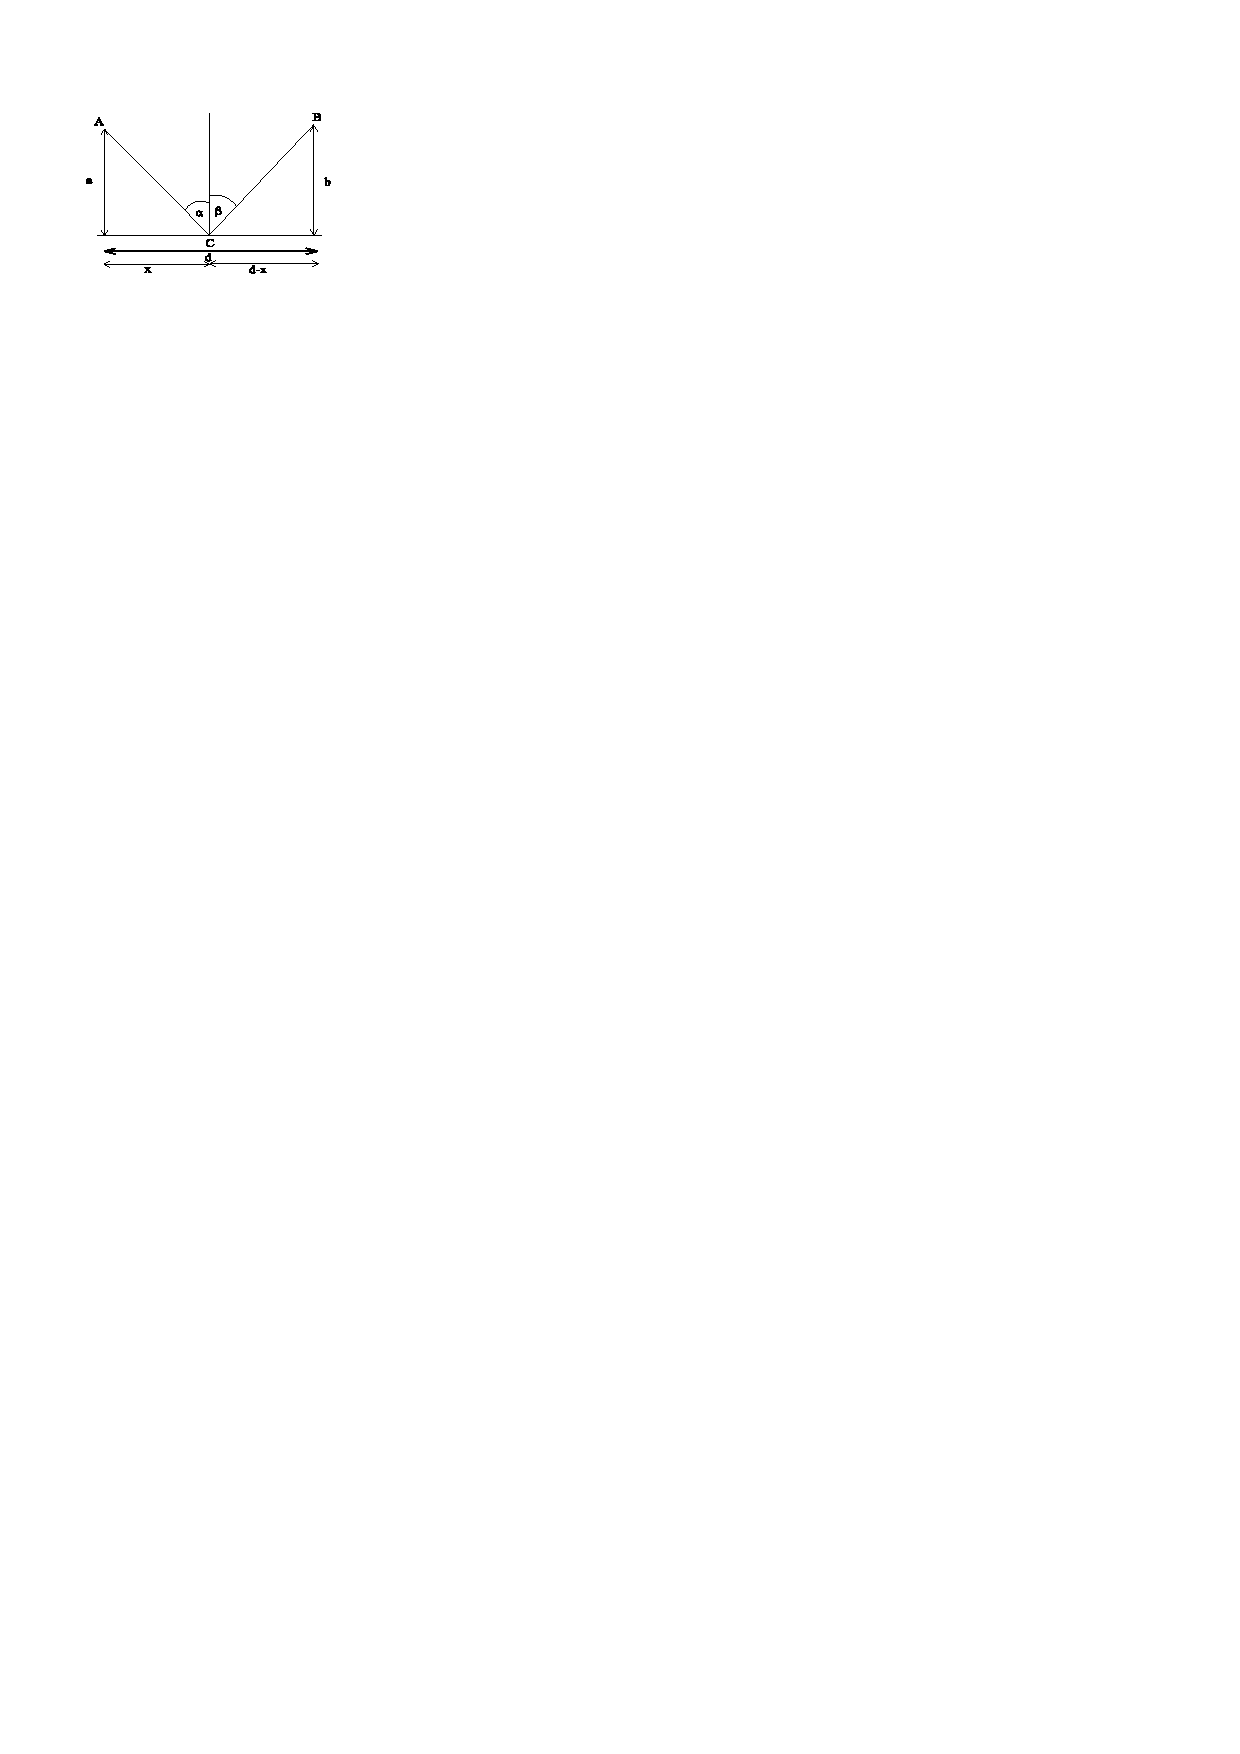
\includegraphics{refleksija_svjetlosti.pdf}
  \caption{Reflekcija svjetlosti}
  \label{refleksija_svjetlosti}
\end{figure}
$$t_{AB} = \int\limits_A^B {\frac{n}{c} dl} = \frac{n}{c} \left (\overline {AC} + \overline {CB} \right) = \frac{n}{c} \left ( \sqrt{a^2+x^2}+\sqrt{b^2+(d-x)^2} \right)$$
Iz Fermatovog principa $\delta t_{AB} = 0$, te imamo:
$$\frac{d}{dx} \left [ \frac{n}{c} \left (\sqrt{a^2 + x^2} + \sqrt{b^2 + (d-x)^2} \right ) \right ] = 0$$
$$\frac{n}{c} \left ( \frac{2x}{2\sqrt{a^2 + x^2}} + \frac{2(d-x)(-1)}{2\sqrt{b^2 + (d-x)^2}} \right ) = 0$$
$$\frac{x}{\sqrt{a^2 + x^2}} = \frac{d-x}{\sqrt{b^2 + (d-x)^2}}$$
$$\sin \alpha = \frac{x}{\overline{AC}} = \frac{x}{\sqrt{a^2 + x^2}}, \ \ \ \sin \beta = \frac{d-x}{\overline{BC}} = \frac{d-x}{\sqrt{b^2+(d-x)^2}}$$
$$\sin \alpha = \sin \beta \Rightarrow \alpha = \beta$$
Dobili smo da je upadni kut jednak kutu refleksije.

\subsection{Fermatov princip i lom svjetlosti}
\begin{figure}[htb!]
	\centering%
	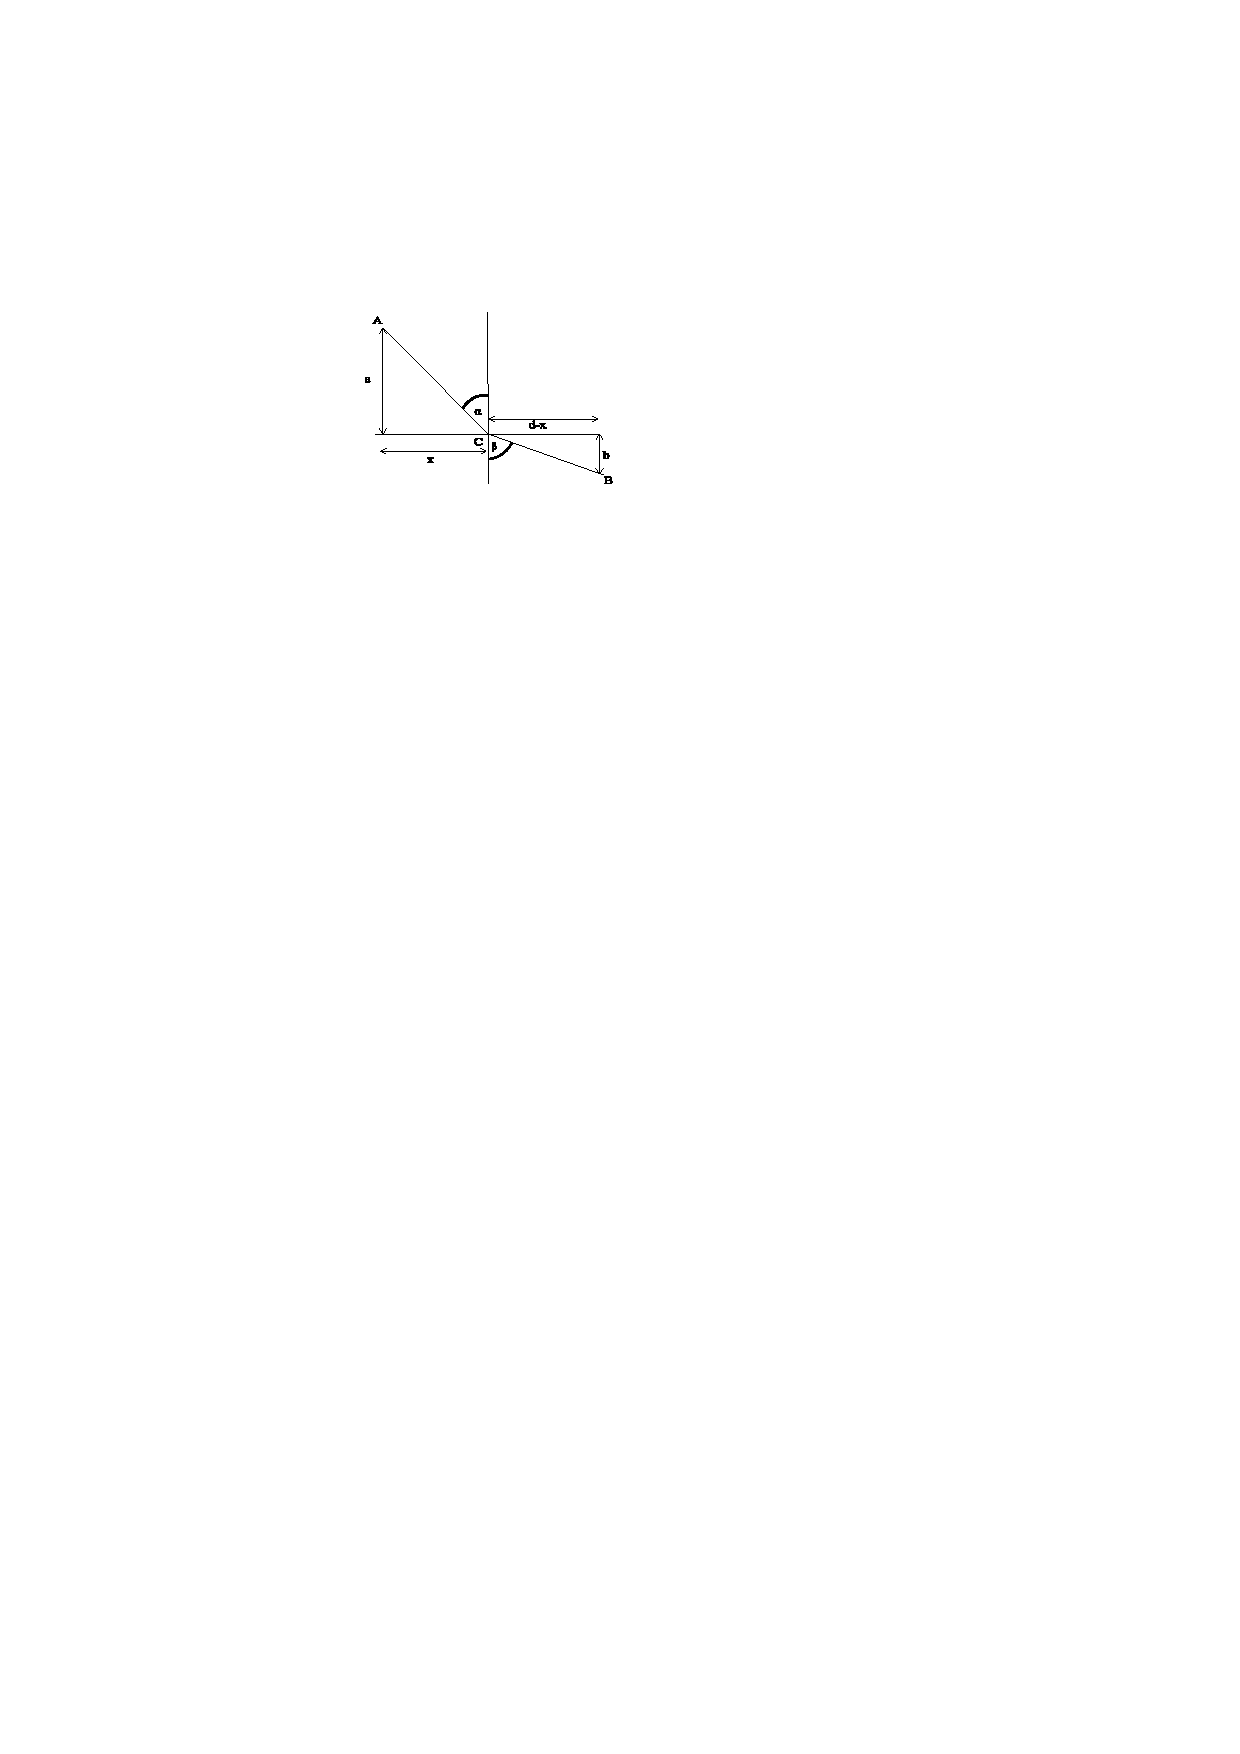
\includegraphics{lom_svjetlosti.pdf}
  \caption{Lom svjetlosti}
  \label{lom_svjetlosti}
\end{figure}
$$t_{AB} = t_{AC} + t_{CB} = \frac{\overline{AC}}{v_1} + \frac{\overline{CB}}{v_2} = \frac{\sqrt{a^2 + x^2}}{v_1} + \frac{\sqrt{b^2 + (d-x)^2}}{v_2}$$
$$\frac{d t_{AB}}{dx} = \frac{1}{v_1} \cdot \frac{2x}{2\sqrt{a^2 + x^2}} + \frac{1}{v_2} \cdot \frac{2(d-x)(-1)}{2\sqrt{b^2+(d-x)^2}} = 0$$
$$\begin{array}{*{20}c}
   {\sin \alpha  = \frac{x}
{{\sqrt {a^2  + x^2 } }}} & {\sin \beta  = \frac{{d - x}}
{{\sqrt {b^2  + (d - x)^2 } }}}  \\
 \end{array} $$
$$\frac{\sin \alpha}{v_1} = \frac{\sin \beta}{v_2} \Rightarrow \frac{n_1}{c} \sin \alpha = \frac{n_2}{c}\sin \beta$$
$$n_1 \sin \alpha = n_2 \sin \beta$$
\begin{center}
	\fbox{$\frac{\sin \alpha}{\sin \beta} = \frac{n_2}{n_1}$}
\end{center}
Snellov zakon loma.

\section{Sferno zrcalo}
\textsc{NAPOMENA:} \textbf{Potrebno je nacrtati sliku!} (Kulišić, (str. 205.; slika 5.12) i (str. 206.; slika 5.13))
\begin{figure}[htb!]
	\centering%
	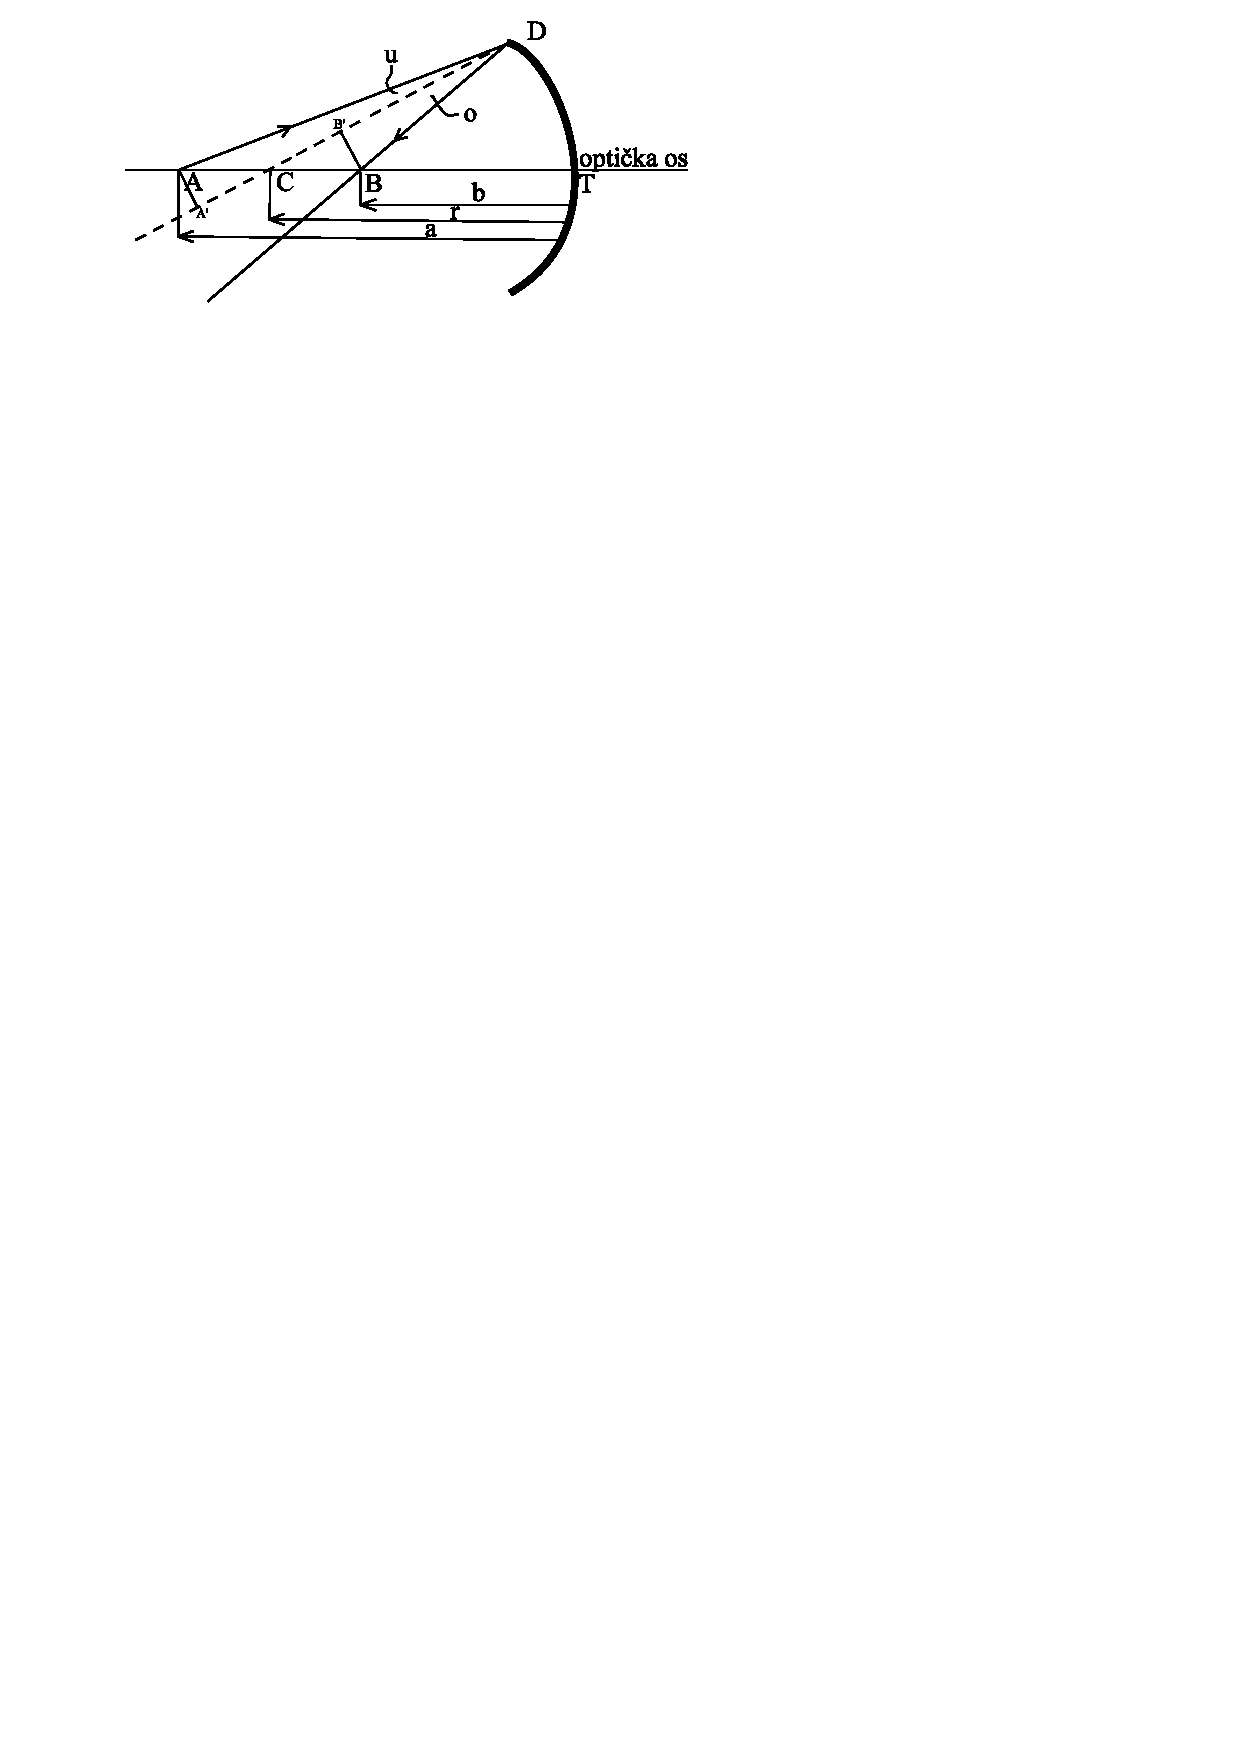
\includegraphics{sferno_zrcalo.pdf}
  \caption{Sferno zrcalo}
  \label{sferno_zrcalo}
\end{figure}

\noindent $T$ - Tjeme zrcala.\\*
$C$ - Središte zakrivljenosti plohe zrcala.
$$\vartriangle AA'C \cong \vartriangle BB'C$$
$$\vartriangle AA'D \cong \vartriangle BB'D$$
$$\begin{array}{*{20}c}
   {\frac{{\overline {AA'} }}
{{\overline {AC} }} = \frac{{\overline {BB'} }}
{{\overline {BC} }}} \hfill & i \hfill & {\frac{{\overline {AA'} }}
{{\overline {AD} }} = \frac{{\overline {BB'} }}
{{\overline {BD} }}} \hfill &  \Rightarrow  \hfill & {\frac{{\overline {AD} }}
{{\overline {AC} }} = \frac{{\overline {BD} }}
{{\overline {BC} }}} \hfill  \\

 \end{array} $$
Ograničimo se samo na zrake za koje vrijedi Gaussova aproksimacija, odnosno:
$$\overline{AD} \cong \overline{AT} \ \ i \ \ \overline{BD} \cong \overline{BT}$$
Zbog toga jednadžba dobiva oblik:
$$\frac{\overline{AC}}{\overline{AT}} = \frac{\overline{BC}}{\overline{BT}}$$
$\overline{AT} = a$ - Predmetna duljina.\\*
$\overline{BT} = b$ - Slikovna duljina.\\*
$\overline{CT} = r$ - Polumjer zakrivljenosti zrcala.\\*
Koristeći te oznake, jednadžba dobiva oblik:
$$\frac{a}{a-r} = \frac{b}{r-b}$$
$$a(r-b) = b(a-r)$$
$$ar - ab = ba - br$$
Sve dijelimo sa $abr$
$$\frac{1}{b} - \frac{1}{r} = \frac{1}{r} - \frac{1}{a}$$
\begin{center}
	\fbox{$\frac{1}{b} + \frac{1}{a} = \frac{2}{r}$}
\end{center}
To je jednadžba sfernog zrcala.

\subsection{Žarišta sfernog zrcala - predmetno žarište Fa}

Ako stavimo svijetli predmet u predmetno žarište ($F_a$), zrake će se širiti paralelno optičkoj osi (slika je beskonačno daleka tjemenu zrcala).\\*
$\overline{F_a T} = f_a$ - Predmetna žarišna duljina.
$$a = f_a \ \ \ i \ \ \ b \to \infty $$
$$\frac{1}{f_a} + \frac{1}{\infty} = \frac{2}{r}$$
$$f_a = \frac{r}{2}$$

\subsection{Žarišta sfernog zrcala - slikovno žarište Fb}

Ako stavimo svijetli predmet u beskonačno daleku točku, nakon refleksije, zrake će se sjeći u slikovnom žarištu ($F_b$).\\*
$\overline{F_b T} = f_b$ - Slikovna žarišna duljina.
$$a \to \infty \ \ \ i \ \ \ b = f_b$$
$$\frac{1}{\infty} + \frac{1}{f_b} = \frac{2}{r}$$
$$f_b = \frac{r}{2}$$

\subsection{Žarišta sfernog zrcala - žarište}

Žarišna duljina:
$$f_a = f_b = f$$
$$\frac{f}{a} + \frac{f}{b} = 1$$
\begin{center}
	\fbox{$\frac{1}{a} + \frac{1}{b} = \frac{1}{f}$}
\end{center}

\textsc{Dogovor o predznacima:}\\*
Ako su $A$, $B$, i $C$ lijevo od $T$ $\to $ $a > 0$, $b > 0$ i $r > 0$ $\Rightarrow $ predmet i slika su realni $\Rightarrow $ zrcalo je udubljeno.\\*
Ako su $A$, $B$, i $C$ desno od $T$ $\to $ $a < 0$, $b < 0$ i $r < 0$ $\Rightarrow $ predmet i slika su virtualni $\Rightarrow $ zrcalo je izbočeno.

\section{Planparalelna ploča}
\textsc{NAPOMENA:} \textbf{Izvod nema smisla bez slike!} (Kulišić, str. 214.; slika 5.30)
\begin{figure}[htb!]
	\centering%
	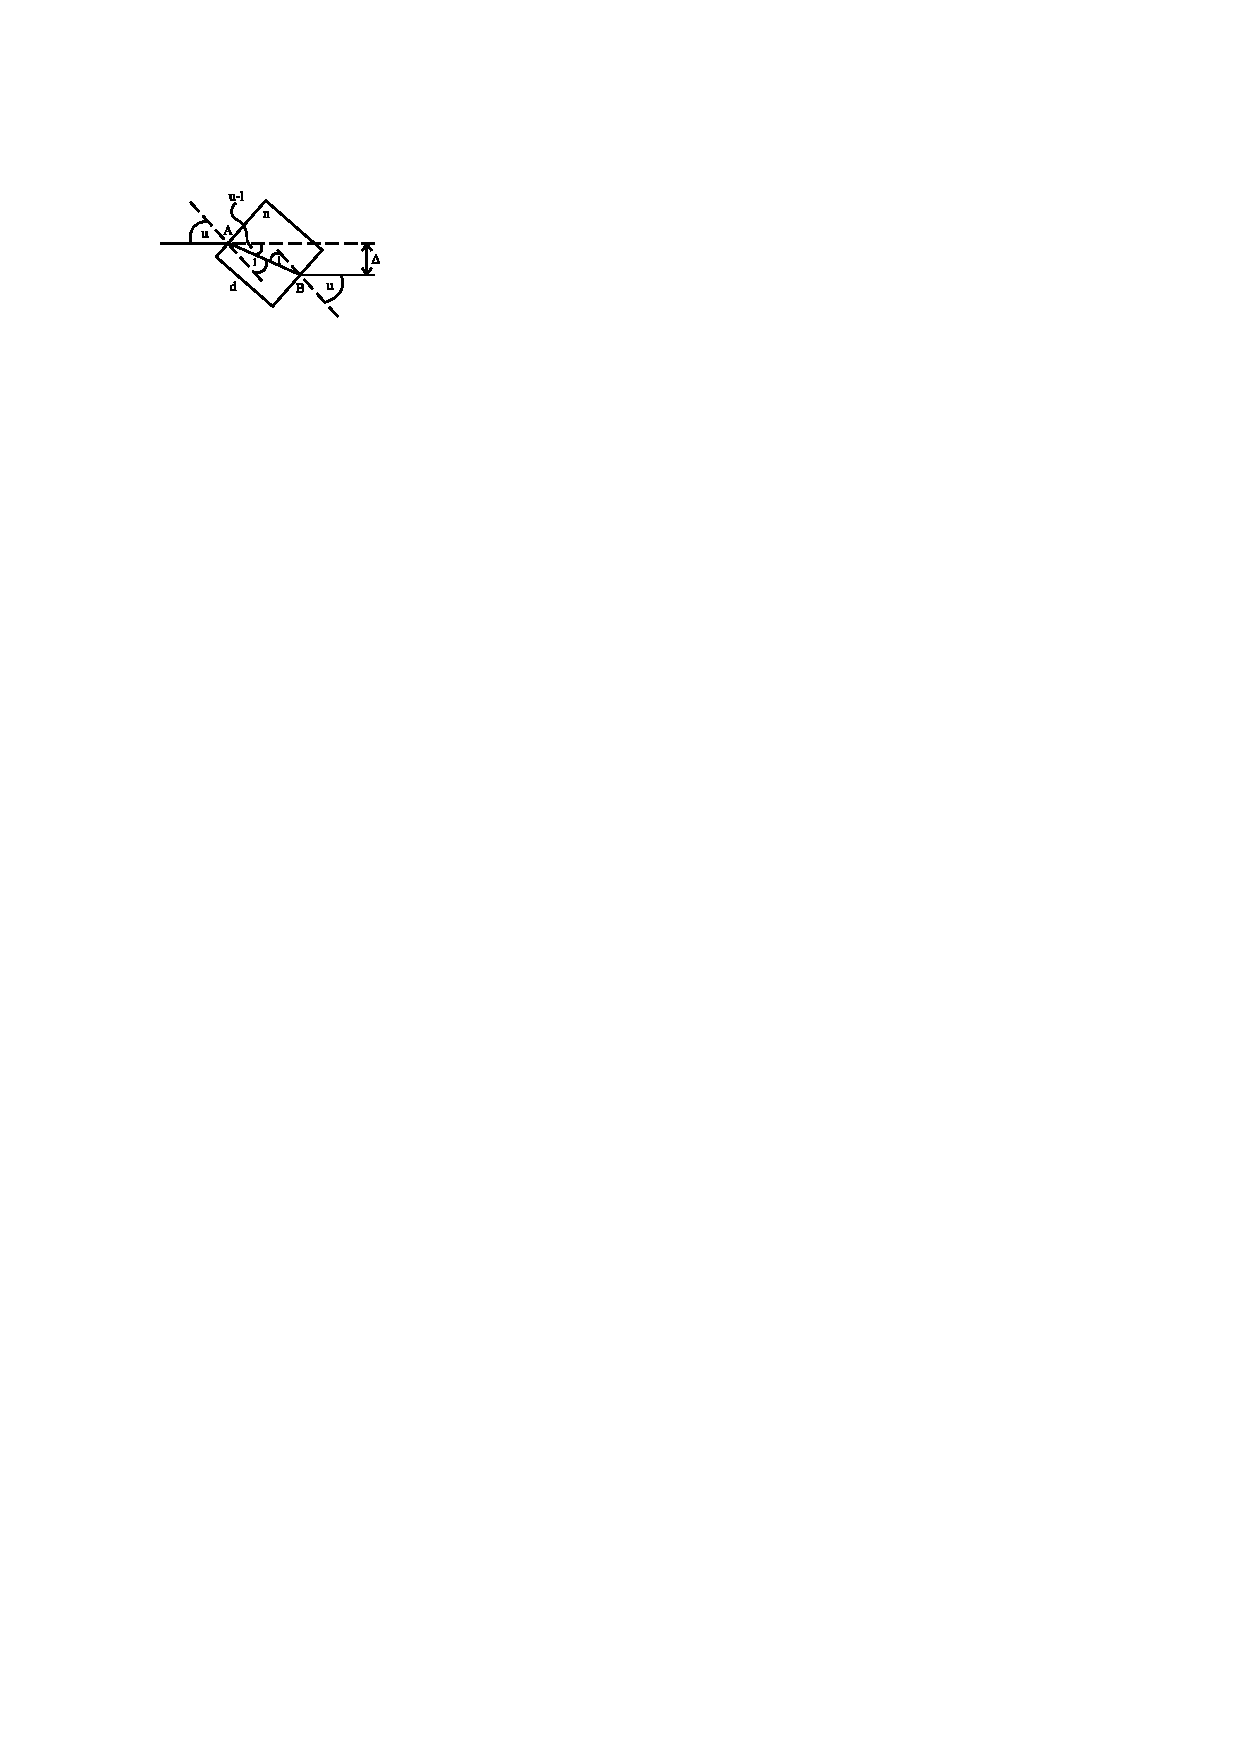
\includegraphics[scale=1.5]{planparalelna.pdf}
  \caption{Planparalelna ploča}
  \label{planparalelna_ploca}
\end{figure}

\noindent $n$ - Indeks loma sredstva od kojeg je načinjena ploča.\\*
$d$ - Debljina ploče.\\*
$u$ - Upadni kut.\\*
$l$ - Kut loma
$$\begin{array}{*{20}c}
   {\sin (u - l) = \frac{\Delta }
{{\overline {AB} }}} & {\cos l = \frac{d}
{{\overline {AB} }}}  \\

 \end{array} $$

$$\Delta = \overline{AB} \sin (u - l) = \frac{d}{\cos l} \cdot \sin (u-l)$$
Snellov zakon loma: $\frac{\sin u}{\sin l} = n$, $\sin l = \frac{\sin u}{n} \Rightarrow \cos l = \sqrt{1 - \frac{\sin ^2 u}{n^2}}$
$$\sin (u-l) = \sin u \cos l - \cos u \sin l$$
$$\Delta = \frac{d}{\cos l} (\sin u \cos l - \cos u \sin l) = d \left (\sin u - \cos u \frac{\sin u}{n\cos l} \right ) =$$
$$= d \sin u \left (1 - \frac{\cos u}{n\sqrt{1 - \frac{\sin ^2 u}{n^2}}} \right ) = d \sin u \left (1 - \frac{\cos u}{\sqrt{n^2 - \sin ^2 u}} \right )$$

\section{Lom svjetlosti na sfernoj granici}
\textsc{NAPOMENA:} \textbf{Izvod nema smisla bez slike!} (Kulišić, str. 220.; slika 5.32)
\begin{figure}[htb!]
	\centering%
	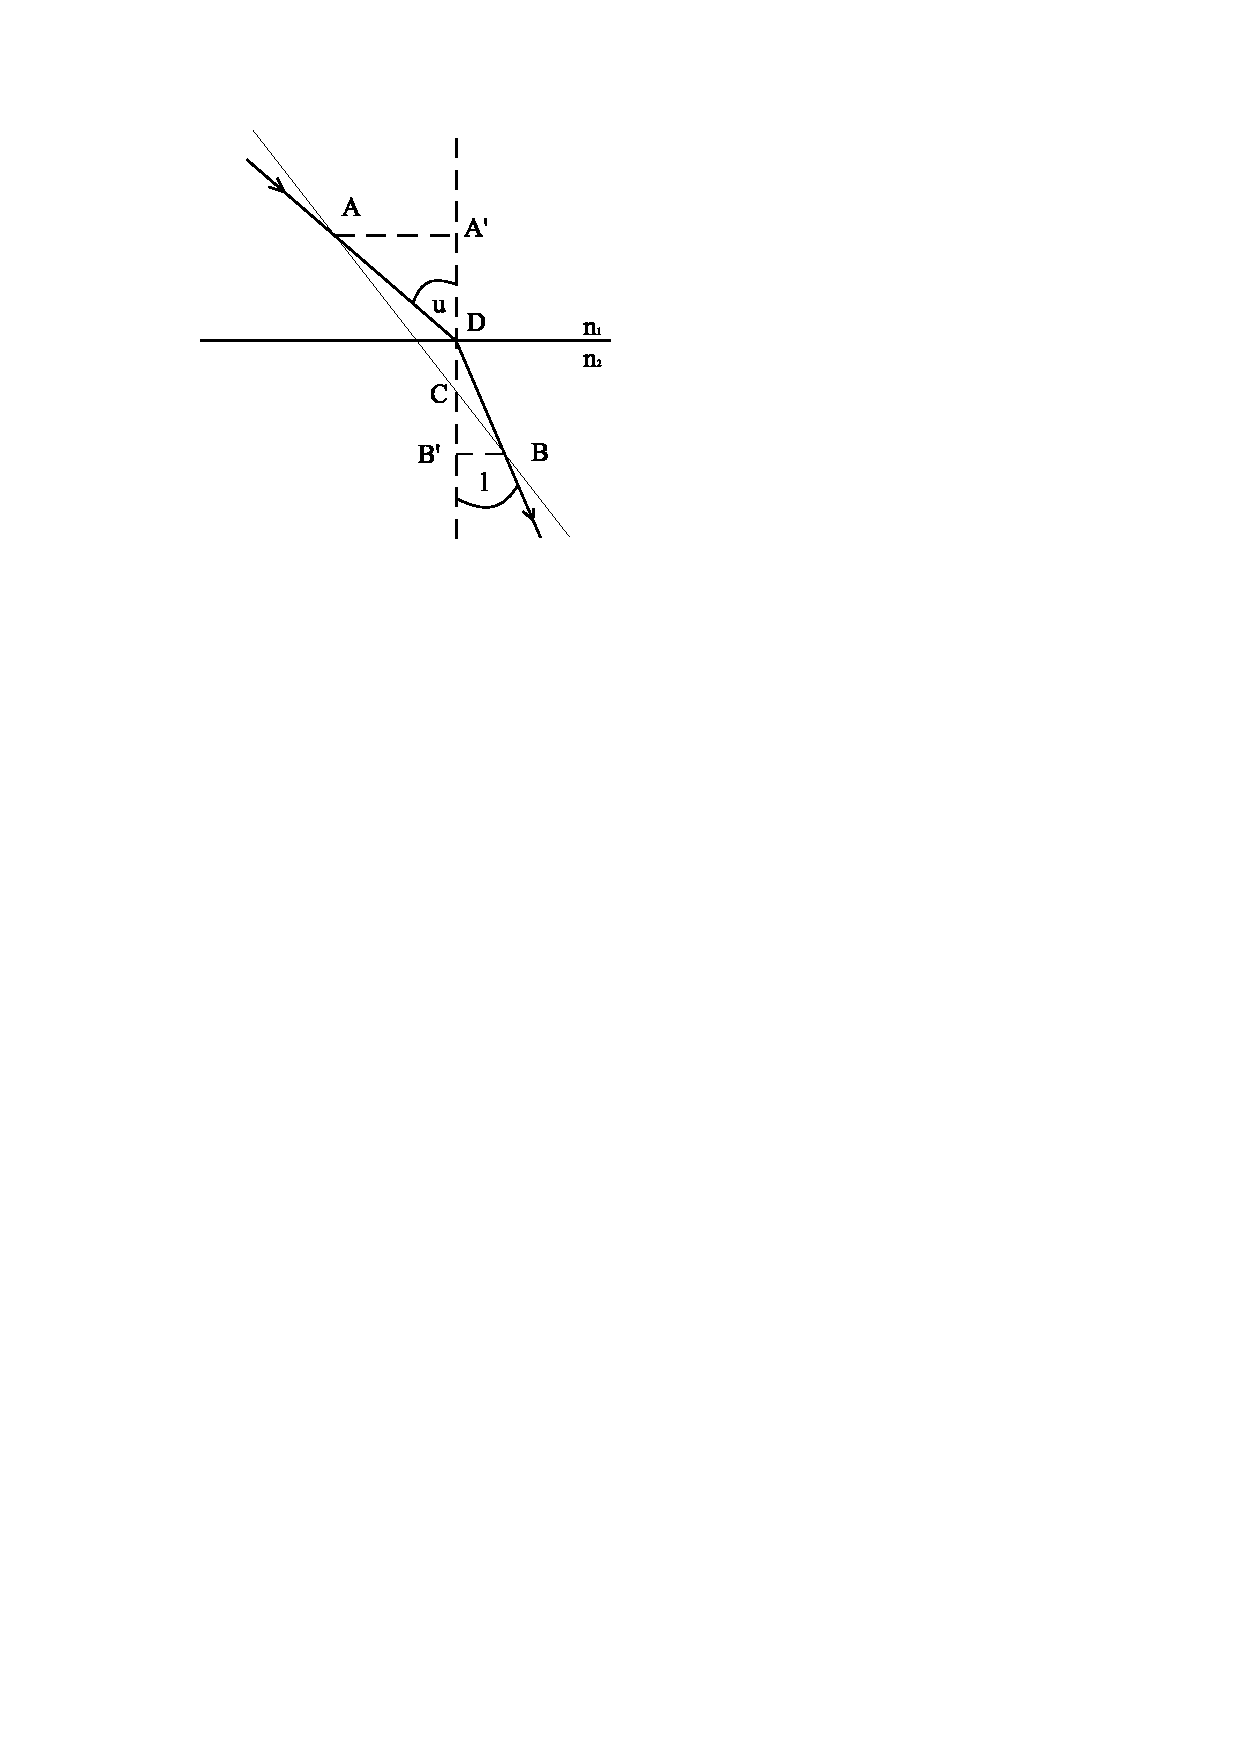
\includegraphics[scale=0.65]{lom_na_sfernoj_granici.pdf}
  \caption{Lom svjetlosti na sfernoj granici}
  \label{lom_na_sf_gran}
\end{figure}

\textsc{M\"{o}biusov oblik}:\\*
Imamo dva slična pravokutna trokuta $\triangle AA'C$ i $\triangle BB'C$ za čije stranice vrijedi:
$$\frac{\overline{AC}}{\overline{AA'}} = \frac{\overline{BC}}{\overline{BB'}}$$
Iz trokuta $\triangle AA'D$ i $\triangle BB'D$ imamo:
$$\overline{AA'} = \overline{AD} \sin u$$
$$\overline{BB'} = \overline{BD} \sin l$$
Iz toga dobivamo:
$$\frac{\overline{AC}}{\overline{AD} \sin u} = \frac{\overline{BC}}{\overline{BD} \sin l}$$
Iz Snellovog zakona, $n_1 \sin u = n_2 \sin l$ i gornjeg izraza, dobivamo:
\begin{center}
	\fbox{$n_1 \frac{\overline{AC}}{\overline{AD}} = n_2 \frac{\overline{BC}}{\overline{BD}}$}
\end{center}
To je zakon loma svjetlosti u M\"{o}biusovom obliku.

\section{Zakon loma na sfernoj granici}

$$n_1 \frac{\overline{AC}}{\overline{AD}} = n_2 \frac{\overline{BC}}{\overline{BD}}$$
Gaussove aproksimacije:
$$\left. {\begin{array}{*{20}c}
   {\overline {AD}  \simeq \overline {AT} }  \\
   {\overline {BD}  \simeq \overline {BT} }  \\
   {\overline {CD}  \simeq \overline {CT} }  \\

 \end{array} } \right\}n_1 \frac{{\overline {AC} }}
{{\overline {AT} }} = n_2 \frac{{\overline {BC} }}
{{\overline {BT} }}$$
$\overline{AT} = a$ - Predmetna daljina.\\*
$\overline{BT} = b$ - Slikovna daljina.\\*
$\overline{CT} = r$ - Polumjer zakrivljenosti sferne granice.
$$\left. {\begin{array}{*{20}c}
   {\overline {AC}  = a + r}  \\
   {\overline {BC}  = b - r}  \\

 \end{array} } \right\}n_1 \frac{{a + r}}
{a} = n_2 \frac{{b - r}}
{b}$$
\begin{center}
	\fbox{$\frac{n_1}{a} + \frac{n_2}{b} = \frac{n_2 - n_1}{r}$}
\end{center}
Zakon loma na sfernoj granici.

Dogovor o predznacima:\\*
Ako je $A$ lijevo od $T$, $a > 0$, predmet je realan. U protivnome, predmet je virtualan.\\*
Ako je $B$ desno od $T$, $b > 0$, slika je realna. U protivnome, slika je virtualna.

\section{Jednadžba tanke leće}
\textsc{NAPOMENA:} \textbf{Izvod nema smisla bez slike.} (Kulišić, (str. 226.; slika 5.42))
\begin{figure}[htb!]
	\centering%
	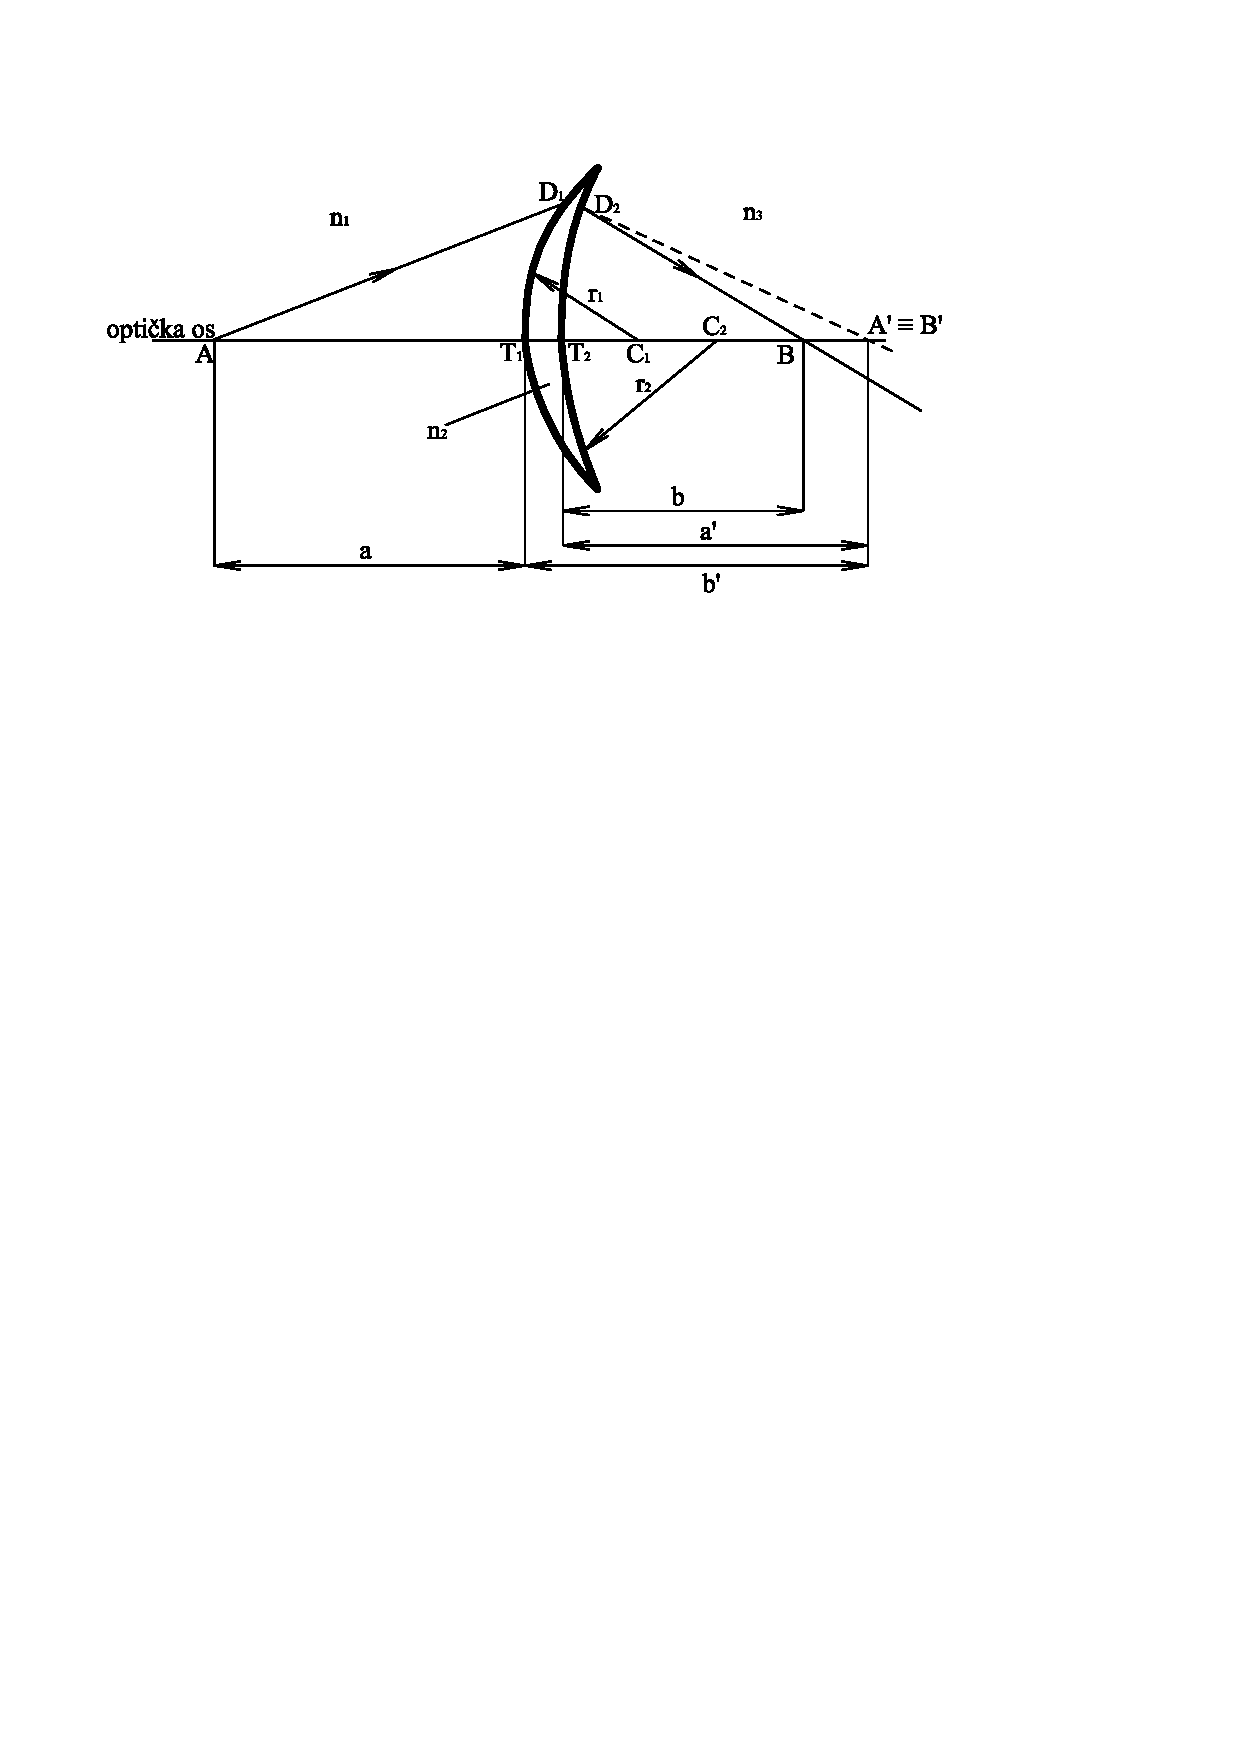
\includegraphics[scale=0.55]{leca.pdf}
  \caption{Leća}
  \label{leca}
\end{figure}

Imamo svijetli predmet u točki $A$.\\*
$\overline{AT_1} = a$ - Predmetna udaljenost.\\*
$\overline{T_2B} = b$ - Slikovna udaljenost.\\*
$\overline{T_1B'} = b'$\\*
$b' \to a' + \overline{T_1 T_2}$\\*
$\overline{T_1B'} = a'$\\*
$b' = a' + \overline{T_1 T_2} = b'$

\textsc{Lom na prvoj sfernoj granici:}

$A\xrightarrow{{n_1 }}D_1 \xrightarrow{{n_2 }}B'$\\*
Uz Gaussove aproksimacije imamo:
$$\frac{n_1}{a} + \frac{n_2}{b'} = \frac{n_2 - n_1}{r_1}$$

\textsc{Lom na drugoj sfernoj granici:}

$B'\xrightarrow{{n_2 }}D_2 \xrightarrow{{n_3 }}B$\\*
Uz Gaussove aproksimacije imamo:
$$\frac{n_2}{a'} + \frac{n_3}{b} = \frac{n_3 - n_2}{r_2}$$
\textsc{Tanka leća} $\rightarrow $ $\overline{T_1 T_2} \approx 0$, $\left| {b'} \right| = \left| {a'} \right|$\\*
$A' \equiv B'$ desno od sferne granice $a' < 0$, $b' > 0$, $a' = -b'$.
$$\frac{n_1}{a} + \frac{n_2}{b'} = \frac{n_2 - n_1}{r_1} \Rightarrow \frac{n_2}{b'} = \frac{n_2 - n_1}{r_1} - \frac{n_1}{a}$$
$$\frac{-n_2}{b'} + \frac{n_3}{b} = \frac{n_3 - n_2}{r_2} \Rightarrow \frac{n_2}{b'} = \frac{n_3}{b} - \frac{n_3 - n_2}{r_2}$$
$$\frac{n_2 - n_1}{r_1} - \frac{n_1}{a} = \frac{n_3}{b} - \frac{n_3 - n_2}{r_2}$$
\begin{center}
	\fbox{$\frac{n_1}{a} + \frac{n_3}{b} = \frac{n_2 - n_1}{r_1} + \frac{n_3 - n_2}{r_2}$}
\end{center}
Jednadžba tanke leće.

\section{Žarište leće}

$$T_1 = T_2 = T$$
\textsc{Predmetno žarište} $F_a$\\*
Predmetna žarišna duljina $f_a = \overline{F_a T}$.
$$\begin{array}{*{20}c}
   {a \to f_a } & {b \to \infty }  \\

 \end{array} $$
$$\frac{n_1}{f_a} + \frac{n_3}{\infty} = \frac{n_2 - n_1}{r_1} + \frac{n_3 - n_2}{r_2}$$
$$f_a = \frac{n_1 r_1 r_2}{r_2 (n_2 - n_1) + r_1 (n_3 - n_2)}$$

\noindent \textsc{Slikovno žarište} $F_b$\\*
Slikovna žarišna duljina $f_b = \overline{F_b T}$.
$$\begin{array}{*{20}c}
   {a \to \infty } & {b \to f_b }  \\

\end{array} $$
$$\frac{n_1}{\infty} + \frac{n_3}{f_b} = \frac{n_2 - n_1}{r_1} + \frac{n_3 - n_2}{r_2}$$
$$f_b = \frac{n_3 r_1 r_2}{r_2 (n_2 - n_1) + r_1 (n_3 - n_2)}$$

$$\frac{f_b}{f_a} = \frac{n_3}{n_1}$$
\begin{center}
	\fbox{$\frac{f_a}{a} + \frac{f_b}{b} = 1$}
\end{center}

\subsection{Tanka leća u zraku}

$$n_1 = n_3 = 1$$
Iz $\frac{f_b}{f_a} = \frac{n_3}{n_1} \Rightarrow f_a = f_b = f$.
$$\frac{1}{f} = \frac{n_2 - n_1}{n_1} \left ( \frac{1}{r_1} - \frac{1}{r_2} \right )$$
$$\frac{f}{a} + \frac{f}{b} = 1$$
\begin{center}
	\fbox{$\frac{1}{a} + \frac{1}{b} = \frac{1}{f}$}
\end{center}

\section{Optička prizma}
\textsc{NAPOMENA:} \textbf{Izvod nema smisla bez slike.} (Kulišić, (str. 215.; slika 5.31))
\begin{figure}[htb!]
	\centering%
	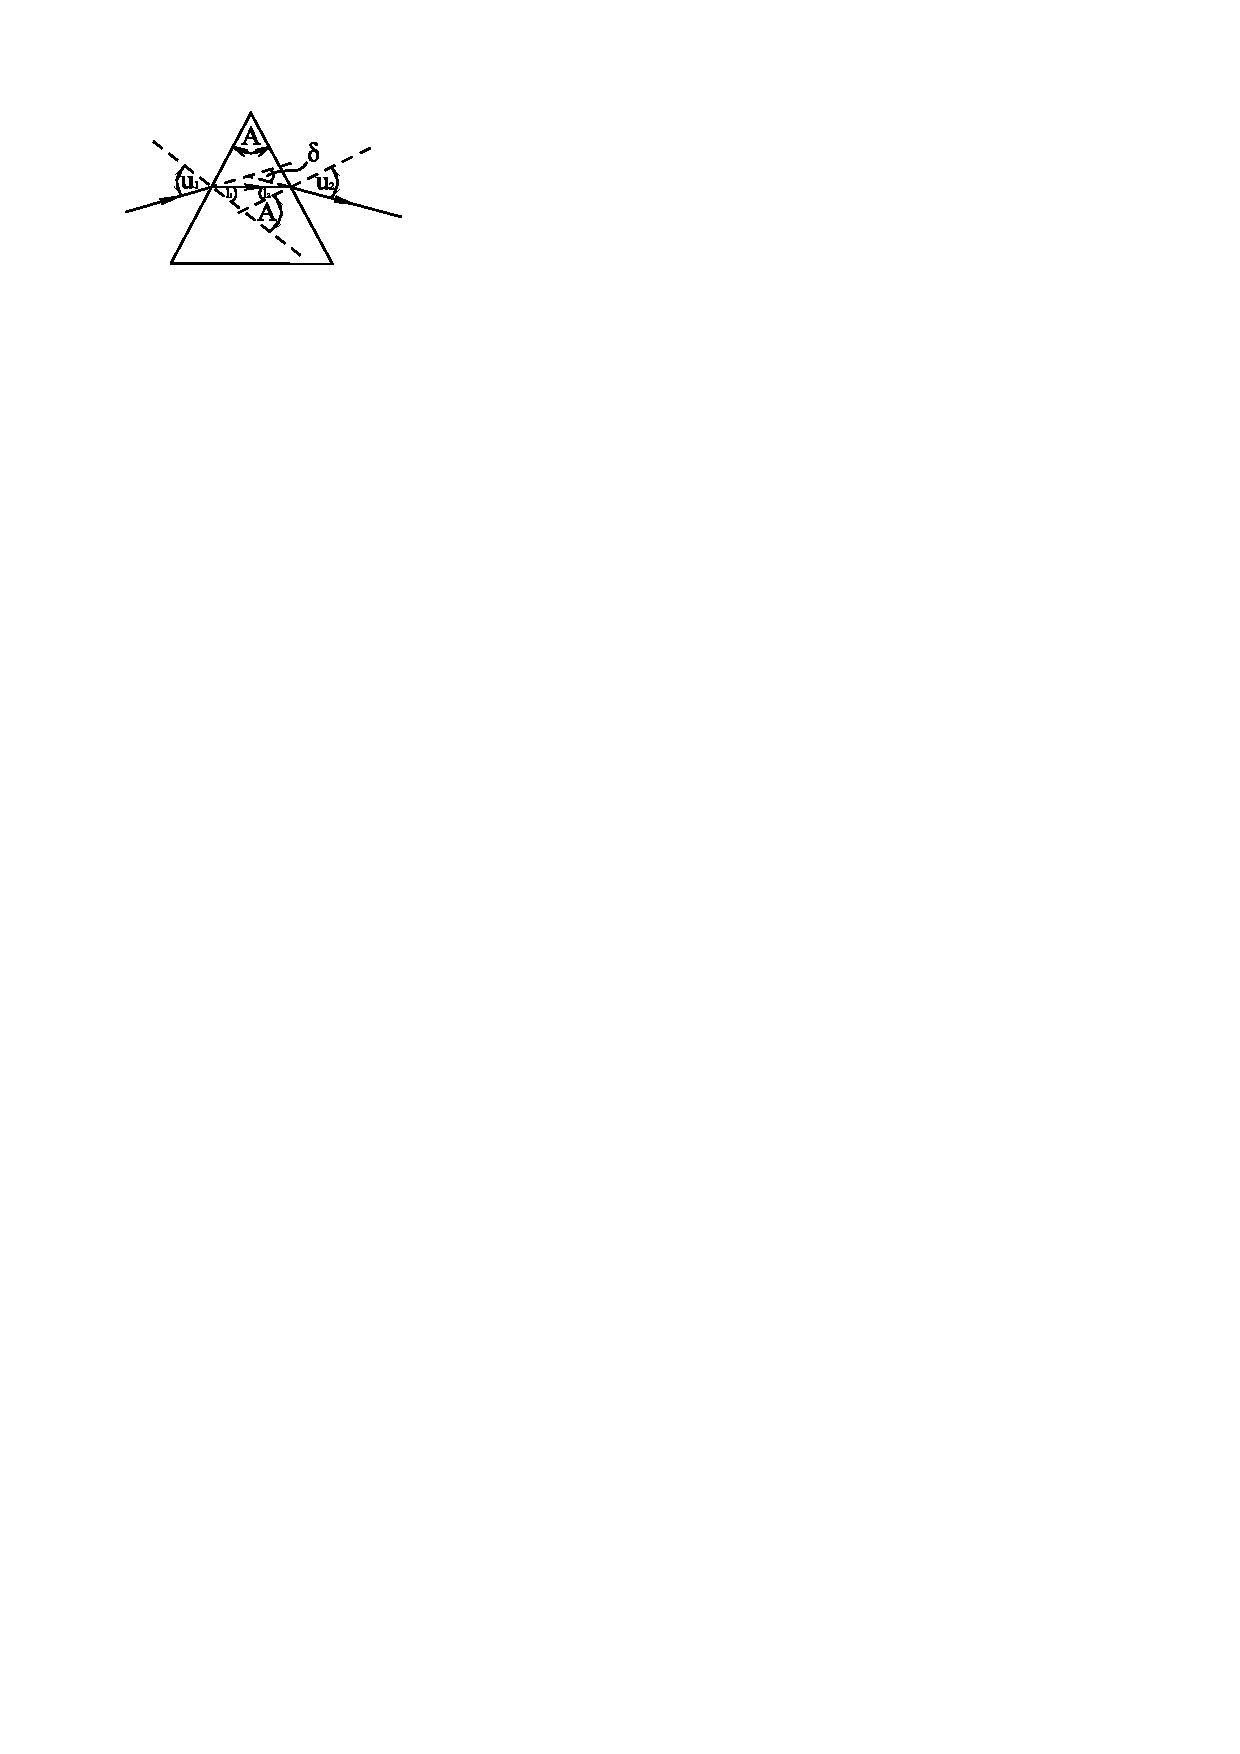
\includegraphics[scale=1.2]{prizma.pdf}
  \caption{Prizma}
  \label{prizma}
\end{figure}

Lomni kut prizme $A$.\\*
$\delta _1 = u_1 - l_1$ - Devijacija upadne zrake.\\*
$\delta _2 = u_2 - l_2$ - Devijacija izlazne zrake.\\*
Ukupna devijacija:
$$\delta = \delta _1 + \delta _2 = u_1 - l_1 + u_2 - l_2 = u_1 + u_2 - (l_1 + l_2)$$
$A = l_1 + l_2 = konst.$ za svaki upadni kut.
$$\delta = u_1 + u_2 - A$$
$$\frac{d\delta}{d u_1} = 0 \Rightarrow \frac{d \delta}{d u_1} = \frac{du_1}{du_1} + \frac{du_2}{du_1} - \frac{dA}{du_1} = 1+\frac{du_2}{du_1} - 0 = 1+\frac{du_2}{du_1}$$
Pretpostavili smo da su sve derivacije funkcije $u_1$.
$$\frac{d \delta}{du_1} = 1 + \frac{du_2}{du_1}$$

\subsection{Snellov zakon loma}

\noindent $\sin u_1 = n \sin l_1$ deriviramo po $u_1$, te imamo:
\begin{equation}
	\cos u_1 = n \cos l_1 \frac{dl_1}{du_1}
	\label{snellov-zakon-01}
\end{equation}

\noindent $l_1 + l_2 = A$ deriviramo po $u_1$
\begin{equation}
	\frac{dl_1}{du_1} + \frac{dl_2}{du_1} = 0
	\label{snellov-zakon-02}
\end{equation}

\noindent $n \sin l_2 = \sin u_2$ deriviramo po $u_1$
\begin{equation}
	n \cos l_2 \frac{dl_2}{du_1} = \cos u_2 \frac{du_2}{du_1}
	\label{snellov-zakon-03}
\end{equation}

\noindent Iz (\ref{snellov-zakon-01}) imamo: $\frac{dl_1}{du_1} = \frac{1}{n} \cdot \frac{\cos u_1}{\cos l_1}$\\*
Iz (\ref{snellov-zakon-02}) imamo: $\frac{dl_2}{du_1} = - \frac{dl_1}{du_1}$\\*
Iz (\ref{snellov-zakon-02}) imamo: $\frac{du_2}{du_1} = n \frac{\cos l_2}{\cos u_2} \cdot \frac{dl_2}{du_1}$

$$\frac{du_2}{du_1} = -n \frac{\cos l_2}{\cos u_2} \cdot \frac{dl_1}{du_1} = - n \frac{\cos l_2}{\cos u_2} \cdot \frac{1}{n} \frac{\cos u_1}{\cos l_1} = - \frac{\cos l_2 \cos u_1}{\cos u_2 \cos l_1}$$
$$\frac{d \delta}{d u_1} = 0 \Rightarrow 1 + \frac{du_2}{du_1} = 0 \Rightarrow \frac{du_2}{du_1} = -1 \Rightarrow \frac{\cos l_2 \cos u_1}{\cos u_2 \cos l_1} = 1$$
$$\cos l_1 = \sqrt{1-\sin ^2 l_1} = \sqrt{1 - \frac{\sin ^2 u_1}{n^2}}$$
$$\cos l_2 = \sqrt{1 - \sin ^2 l_2} = \sqrt{1 - \frac{\sin ^2 u_2}{n^2}}$$
$$\frac{\cos u_1}{\cos l_1} = \frac{\cos u_2}{\cos l_2}$$
$$\frac{\cos u_2}{\sqrt{1-\frac{\sin ^2 u_1}{n^2}}} = \frac{\cos u_2}{\sqrt{1-\frac{\sin ^2 u_2}{n^2}}}$$
$$\frac{\cos ^2 u_1}{n^2 - \sin ^2 u_1} = \frac{\cos ^2 u_2}{n^2 - \sin ^2 u_2}$$
$$\frac{1-\sin^2 u_1}{n^2 - \sin ^2 u_1} = \frac{1 - \sin ^2 u_2}{n^2 - \sin ^2 u_2}$$
$$(n^2 - 1)(\sin^2 u_2 - \sin ^2 u_1) = 0$$
$$(n^2 - 1) \neq 0 \Rightarrow (\sin^2 u_2 - \sin ^2 u_1) = 0 \Rightarrow u_2 = u_1$$
\begin{center}
	\fbox{$u_2 = u_1$}
\end{center}

\subsection{Simetričan prolaz svjetlosti}
$\delta $ je minimalan:
$$\frac{d^2 \delta}{du^2 _1} > 0$$

\subsection{Indeks loma prizme}

$u_1 = u_2$ za slučaj $\delta = min$.

$$\delta = 2u_1 -A$$
$$A = 2l_1$$
$$u_1 = \frac{1}{2} (\delta _{min} + A)$$
\textsc{Snellov zakon loma:}
$$n = \frac{\sin u_1}{\sin l_1} = \frac{\sin \left ( \frac{\delta _{min} + A}{2} \right )}{\sin \frac{A}{2}}$$


\end{document}
